\section{Pushing the envelope in speed, efficiency and precision}
\label{section_pushing_limit}

\subsection{Smooth is faster}
In "pgfplots" and Tikz it is usually faster to use relatively fewer
points to plot something and to turn on smoothing, rather than having
no smoothing and calculating lots of points (as you might do in Matlab
for instance).  Shown below are two ways to make a semicircle (of
course, the point is not about the semicircle \emph{per se}, it is
simply a stand-in for plotting functions).  
\begin{center}
\lstset{basicstyle=\color{blue!50!black}\small\tt}

\tikzcount
\begin{minipage}{0.5\columnwidth}
\begin{latex}
\begin{tikzpicture}
\begin{axis}[axis lines=none, axis equal]
\addplot[domain=-1:1,"samples=50"] 
                        {sqrt(1-(x)^2)};
\end{axis}
\end{tikzpicture}
\end{latex}
%
\begin{tikzpicture}
\begin{axis}[axis lines=none, axis equal]
\addplot[domain=-1:1,samples=50] 
                        {sqrt(1-(x)^2)};
\end{axis}
\end{tikzpicture}
\end{minipage}%
~~%
\begin{minipage}{0.5\columnwidth}
\begin{latex}
\begin{tikzpicture}
\begin{axis}[axis lines=none,axis equal]
\addplot["samples at ={-1,0,1},smooth,
            tension=1.7"] {sqrt(1-(x)^2)};
\end{axis}
\end{tikzpicture}
\end{latex}
\begin{tikzpicture}
\begin{axis}[axis lines=none,axis equal]
\addplot[samples at ={-1,0,1},smooth,
            tension=1.7] {sqrt(1-(x)^2)};
\end{axis}
\end{tikzpicture}
\end{minipage}
\tikzcount
\end{center}
Probably both pictures are good enough, especially when you remember
our real goal isn't to draw semicircles but to plot other functions,
and for those, a small inaccuracy in shape probably won't be noticeable.

If you want to see more closely how these shapes compare to a ``real''
semicircle, the graphs below will help.  In each case, the red
semicircle is made by asking Tikz to draw an arc using the command
"arc("\meta{angle}:\meta{angle}:\meta{radius}")", which I'll assume is
more or less perfect. The green path on the left (including the thin
black boundary of that path) is made by calculating $\sqrt{1-x^2}$ at
$50$ points.  The right end doesn't quite touch the horizontal, and
both ends have a short straight segment.  The blue path on the right
is made using 3 points and smoothing.  The ends of the path are a
little too far ``in'', and the ``shoulders'' are a little too far out
(as compared to the red arc which I assume is perfect).
\begin{center}
\tikzcount
\begin{tabular}{c}
\scalebox{4}{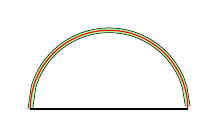
\begin{tikzpicture}
\draw[green, ultra thick, opacity = 0.35,domain=-1:1,samples=50] plot (\x,{sqrt(1-(\x)^2)});
\draw[scale=1.03,very thin, domain=-1:1,samples=50] plot (\x,{sqrt(1-(\x)^2)});
\draw[scale=0.97,very thin, domain=-1:1,samples=50] plot (\x,{sqrt(1-(\x)^2)});
\draw[red](1,0) arc (0:180:1);
\draw (-1,0) -- (1,0);
\end{tikzpicture}}
\\
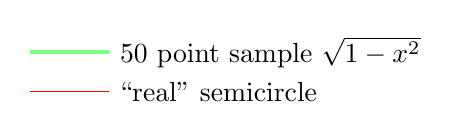
\begin{tikzpicture}
\draw[red] (0,0) -- (1,0) node[right,black]{``real'' semicircle};
\draw[ultra thick, green, opacity= 0.5] (0,0.5) -- (1,0.5)
node[right,black,opacity=1]{50 point sample $\sqrt{1-x^2}$};
\end{tikzpicture}
\end{tabular}%
~~
\tikzcount
\begin{tabular}{c}
\scalebox{4}{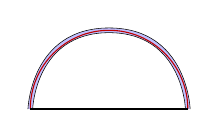
\begin{tikzpicture}
\def\t{1.74}
\draw[ultra thick, opacity = 0.25,domain=-1:1,samples=3,smooth,blue,tension=\t] plot (\x,{sqrt(1-(\x)^2)});
\draw[scale=1.03,very thin,domain=-1:1,samples=3,smooth,tension=\t] plot (\x,{sqrt(1-(\x)^2)});
\draw[scale=0.97,very thin,domain=-1:1,samples=3,smooth,tension=\t] plot (\x,{sqrt(1-(\x)^2)});
\draw[red!75!black](1,0) arc (0:180:1);
\draw (-1,0) -- (1,0);
\end{tikzpicture}}
\\
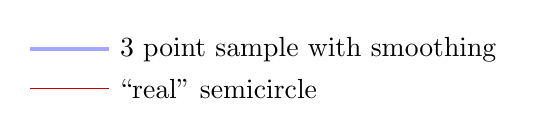
\begin{tikzpicture}
\draw[red!75!black] (0,0) -- (1,0) node[right,black]{``real'' semicircle};
\draw[ultra thick, blue, opacity =0.35] (0,0.5) -- (1,0.5)
node[right,black,opacity=1]{3 point sample with smoothing};
\end{tikzpicture}
\end{tabular}
\end{center}
So we can see some minor imperfections in each case. Maybe which
version you prefer would be a matter of stylistic preference (for me,
I don't like seeing the straight segments on the sample-based
approach).

But the biggest difference between the two approaches is speed.  Making
1000 copies of the first graph took 26 seconds on a MacBook Air~(M1):
% 19s on M4
\begin{latex}
   \foreach \n in {1,2,...,1000}
   {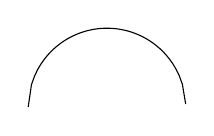
\begin{tikzpicture}
       \draw[domain=-1:1,samples=50] plot (\x,{sqrt(1-(\x)^2)});
     \end{tikzpicture}\linebreak[3]}

\end{latex}
 and this took 2.3 seconds:% 1.7s on M4
\begin{latex}
   \foreach \n in {1,2,...,1000}
   {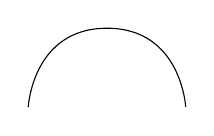
\begin{tikzpicture}
       \draw[samples at ={-1,0,1},smooth,tension=1.7] plot (\x,{sqrt(1-(\x)^2)});
     \end{tikzpicture}\linebreak[3]}

\end{latex}
(Both sets of commands were tested in the command line with 
``"time pdflatex myfile"''.)

This is a rather extreme example, for instance a semicircle only needs
three points but most functions will need more.  And I had to tweak
the tension setting, which I would usually recommend omitting. So, I
wouldn't usually try to use fewer than the default value of 25
samples, but also I would at least consider adding "smooth" to make a
better looking graph before increasing the samples too much.  

So, why not always use smooth? As I said in the beginning of this
guide, I would recommend trying it for a \emph{curve} (though see also
Section~\ref{section_asymptotes} where we saw that "smooth" can
introduce an erroneous wiggle in graphs with asymptotes).  It's not so
good for absolute value:
\begin{center}
\tikzcount
\begin{minipage}{0.55\columnwidth}
\begin{latex}
\begin{tikzpicture}
\begin{axis}[title={plot with smooth}]
\addplot[very thick,"smooth",blue]{abs(x)};
\end{axis}
\end{tikzpicture}%
\end{latex}
%
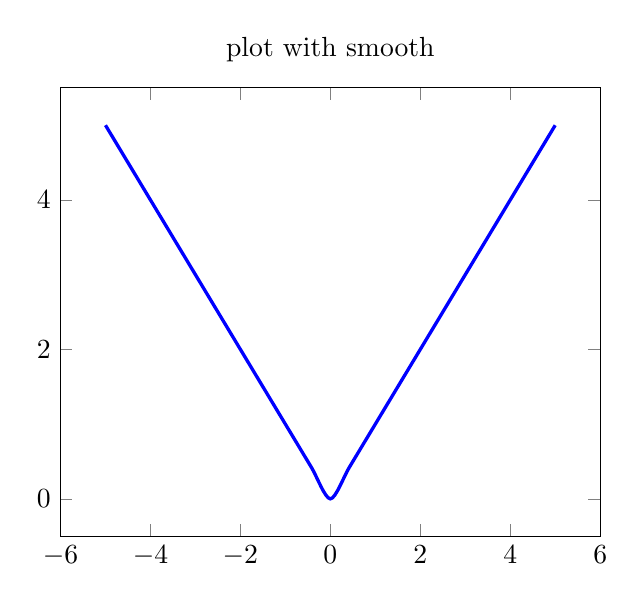
\begin{tikzpicture}
\begin{axis}[title={plot with smooth}]
\addplot[very thick,smooth,blue]{abs(x)};
\end{axis}
\end{tikzpicture}%
\end{minipage}%
~~%
\begin{minipage}{0.45\columnwidth}
\begin{latex}
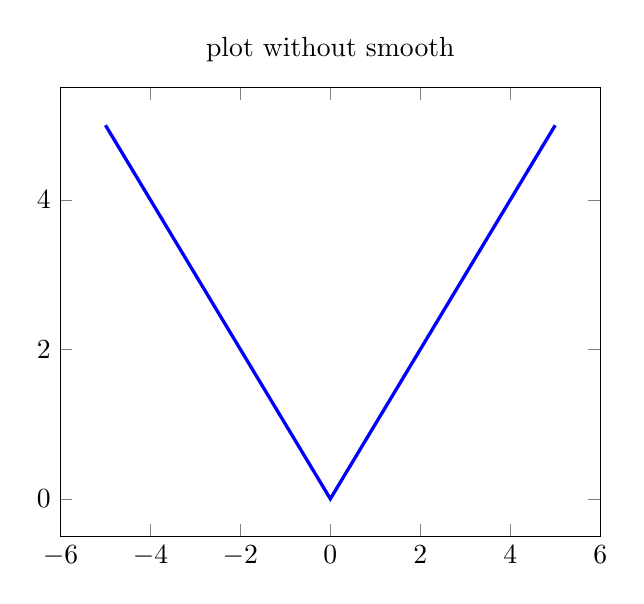
\begin{tikzpicture}
\begin{axis}[title={plot without smooth}]
\addplot[very thick,blue]{abs(x)};
\end{axis}
\end{tikzpicture}
\end{latex}
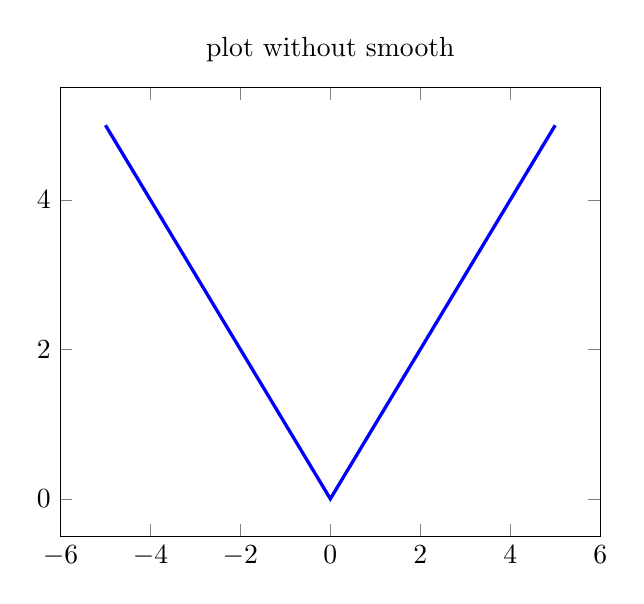
\begin{tikzpicture}
\begin{axis}[title={plot without smooth}]
\addplot[very thick,blue]{abs(x)};
\end{axis}
\end{tikzpicture}%
\end{minipage}
\tikzcount
\end{center}

How do you know when you have reason to increase the number of
samples?  Basically, look at the graph and see what you think.  I find
the square root graph doesn't look correct at the origin with the
standard number of samples:
\begin{latex}
\begin{tikzpicture}
\begin{axis}[axis lines = middle,title={Default samples}]
\addplot[very thick,blue,smooth,domain=0:9]{sqrt(x)};
\end{axis}
\end{tikzpicture}%
~~%
\begin{tikzpicture}
\begin{axis}[axis lines = middle,title={100 Samples}]
\addplot[very thick,blue,smooth,domain=0:9,"samples=100"]{sqrt(x)};
\end{axis}
\end{tikzpicture}
\end{latex}
%
\begin{center}
\tikzcount
\begin{tikzpicture}
\begin{axis}[axis lines = middle,title={Default samples}]
\addplot[very thick,blue,smooth,domain=0:9]{sqrt(x)};
\end{axis}
\end{tikzpicture}%
~~%
\def\numsamples{100}
\tikzcount
\begin{tikzpicture}
\begin{axis}[axis lines = middle,title={\numsamples\ Samples}]
\addplot[very thick,blue,smooth,domain=0:9,samples=\numsamples]{sqrt(x)};
\end{axis}
\end{tikzpicture}
\end{center}
It irks me that I need 100 samples (four times the default) to
(\emph{almost}) make the artifact at the origin go away.  On the other
hand, I need even more points in Matlab, because there's no smoothing
there.  The problem is that the first and second derivatives of
$\sqrt{x}$ are both large at the origin.  If I \emph{really} don't
want to use this many points, I can do a parametric graph and make $y$
the independent variable, and then I can get by with even fewer
samples than the default:
\begin{latex}
\begin{tikzpicture}
\begin{axis}[axis lines = middle,title={15 samples, Parametric plot}]
\addplot[very thick,blue,smooth,domain=0:3,"variable=t","samples=15"]"({t^2},{t})";
\end{axis}
\end{tikzpicture}
\end{latex}
%
\begin{center}
\tikzcount
\begin{tikzpicture}
\begin{axis}[axis lines = middle,title={15 samples, Parametric plot}]
\addplot[very thick,blue,smooth,domain=0:3,variable=t,samples=15]({t^2},{t});
\end{axis}
\end{tikzpicture}
\end{center}

One canonical example of a difficult to graph function is
the so-called topologist's sine curve $y=\sin(1/x)$.  When I plot this
in Matlab, on the interval $[0,4/\pi]$, with its adaptive command "fplot"
the resulting figure uses 1682 $x$-values! 
% f = @(x) sin(1./x)
% ax = fplot(f,[0,4/\pi])
% ax.XData
% shows 1x1682 vector
Can we do better?  How much better?  To do a good job we should have
the $x$-values more densely chosen as $x\to 0^+$.  As is often the
case (maybe always?) a parametric approach works a lot better.  Here's
my final result, and then I'll explain how I got it.
\begin{center}
\tikzcount
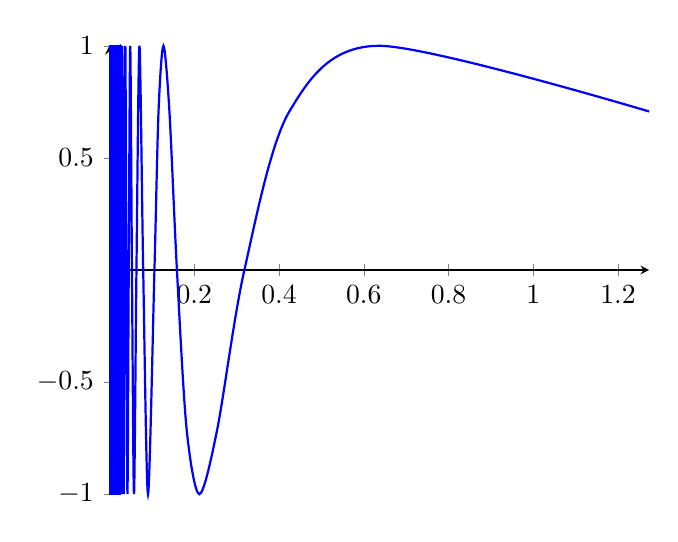
\begin{tikzpicture}
  \begin{axis}[axis lines = middle,xmin=0,clip=false]
    % y-value on rectangle increased to cover the thickness of the
    % line of the sine curve as it "turns the corner"
 \draw[blue,fill=blue] (0,-1.0025) rectangle (0.02546,1.0025);
 \addplot[thick,blue,variable = t, 
         samples at = {
           45, 90, ..., 540, % multiples of 45,
           630, 720, ..., 2250}, % multiples of 90 
         smooth] ({1/rad(t)},{sin(t)}) circle (0.01pt);
\end{axis}
\end{tikzpicture}
\end{center}
To be clear, I worked hard to make that graph as good as I thought it
could be, and to make it as efficient as possible in terms of number
of points that are sampled.  I'm not recommending you work this hard
in general to produce a nice enough looking graph.  

In terms of making it parametric, I replaced $y=\sin(1/x)$ with
$x=1/t$ and $y=\sin(t)$.  This makes it easy to specify $t$-values
that correspond to meaningful parts of the curve, e.g.\
$t=\pi/2, 3\pi/2, 5\pi/2, \dots, (2n+1)\pi/2$ will give us a sequence
of the max and mins of this curve.  Just using these points would give
us a curve that is efficient, simple to describe, and at least matches
the correct max and mins.  In the end, I added some multiples of
$\pi/4$ at the beginning, i.e.\ to produce the right ``half'' of the
curve.  

Now, what about the left end? As we get close enough to the $y$-axis
the blue lines blur together, and at that point I will (1) just draw a
filled blue rectangle, (2) stop calculating values for $\sin(1/x)$
(where ``stop'' means I'm thinking of values moving from the right to
the left.)  Let's find the $x$-value where the blue rectangle should
meet the $\sin(1/x)$ curve.  It should be where two successive peaks
of $\sin(1/x)$ have overlapping lines, so that the separate peaks are
almost indistinguishable from each other.

The lines have thickness 0.8pt (because that's the default value for
"thick" paths), and that's an external dimension, i.e.\ what we should
see if we print this out and measure it.  Thus, two peaks will be
indistinguishable when they have a distance apart, in
internal-axis-dimensions, less than or equal to 0.8pt.  So, what are
the internal dimensions of 0.8pt?  Let's use ``iu'' for internal unit,
i.e.\ the distance from $x=0$ to $x=1$ in the axes.  Then we have (see
Section~\ref{section_sizing_axes})
\begin{align*}
\qty{1.27}{iu} + \qty{45}{pt} & = \qty{240}{pt}\\
 \qty{1.27}{iu} & = \qty{195}{pt}\\
 \qty{0.8}{pt} & = \frac{1.27}{195}\times0.8 \unit{iu}  = \qty{0.0052}{iu}
\end{align*}
In other words, if $x_1$ and $x_2$ are the $x$-values of two
successive peaks, then the peaks would be indistinguishable for
$x_1-x_2 < \qty{0.0052}{iu}$.

So now we ask, what are the first pair of $x$-values that satisfy this
condition? That will tell us the $x$-value for the right edge of the
blue rectangle, and it will tell us what $n$ should be where the peak
occurs at $x=\frac{2}{(4n+1)\pi}$.  Thus we wish to solve the
following
\begin{align*}
\frac{2}{(4n+1)\pi}-\frac{2}{(4n+5)\pi} & < 0.0052\\
\frac{4n+5-(4n+1)}{(4n+1)(4n+5)}  & < \frac{\pi}{2}(0.0052)\\
\frac{(4n+1)(4n+5)}{4}  & > \frac{2}{(0.0052)\pi}\\
(4n+1)(4n+5) & > \frac{8}{(0.0052)\pi}\\
 n & \ge 5.8
\end{align*}
When $n=6$ we find $x = \frac{2}{(4\cdot 6+1)\pi} \approx 0.02564$.
This is the right edge of the blue rectangle we used in the graph
above.  And $n=6$ means that in our parametric plot
$t=(4\cdot 6+1)\pi/2 = 25\pi/2=25\times 90^\circ = 2250^\circ$ is the
last $t$-value we use.  Here's the code
\begin{latex}
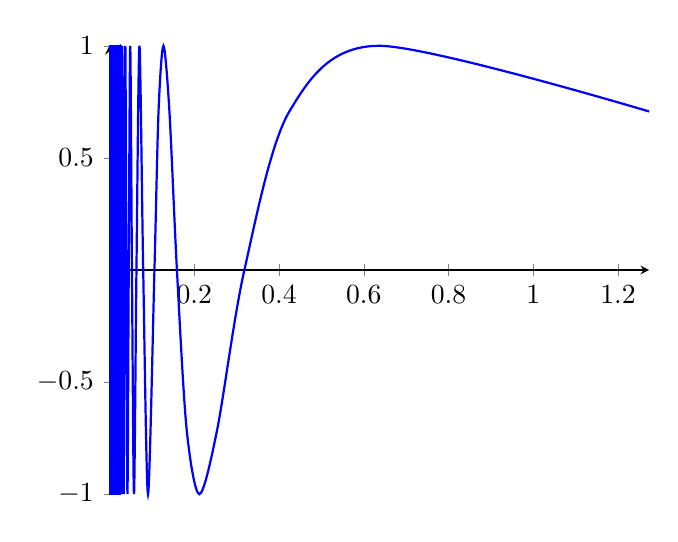
\begin{tikzpicture}
  \begin{axis}[axis lines = middle,xmin=0,clip=false]
    % y-value on rectangle increased to cover the thickness of the
    % line of the sine curve as it "turns the corner"
 \draw[blue,fill=blue] (0,-1.0025) rectangle (0.02546,1.0025);
 \addplot[thick,blue,variable = t, 
         samples at = {
           45, 90, ..., 540, % multiples of 45,
           630, 720, ..., 2250}, % multiples of 90 
         smooth] ({1/rad(t)},{sin(t)}) circle (0.01pt);
\end{axis}
\end{tikzpicture}

\end{latex}
Here's a magnification of the top of the curve right at the
$x=0.02546$ boundary (I've set "opacity=0.5" on both the rectangle and
the sine curve, so we can see how they overlap).  Reading from the
right, we see two peaks on $\sin(1/x)$ that are not tounching the
rectangle, and then the next one is almost entirely covered up by the
blue rectangle:
\begin{center}
\tikzcount
\begin{tikzpicture}[spy using outlines={circle, magnification=15, size=2.5cm, connect spies}]
  \begin{axis}[axis lines = middle,xmin=0,clip=false]
    % y-value on rectangle increased to cover the thickness of the
    % line of the sine curve as it "turns the corner"
 \draw[blue,fill=blue,opacity=0.5] (0,-1.0025) rectangle (0.02546,1.0025);
 \addplot[opacity=0.5,thick,blue,variable = t, 
         samples at = {
           45, 90, ..., 540, % multiples of 45,
           630, 720, ..., 2250}, % multiples of 90 
         smooth] ({1/rad(t)},{sin(t)}) circle (0.01pt);
\end{axis}
\spy[red] on (4.5pt,5.7) in node[left] at (-0.5,6);
\end{tikzpicture}
\end{center}


\subsection{Graphs with a large number of points}
Up to this point I have perhaps overemphasized the goal of being
efficient in how many points we need to sample to make a nice graph.
There are certainly times when we simply have to throw a pretty large
number of points into our computer, and if this does take too long
there are ways to help with that too (see
Section~\ref{section_externalization}).

The following three graphs are interesting examples where I needed to
use 200--300 points to get a result that I thought looked nice:
\begin{center}
\everymath{\displaystyle}
\begin{minipage}{0.5\columnwidth}
\begin{latex}[xleftmargin=0in,
basicstyle=\color{blue!75!black}\small\tt,
]
\begin{tikzpicture}[
declare function = {
f(\x) = (\x-0.5)*sin(1/(\x^2-\x+0.27));
}]
\begin{axis}[axis lines = middle,
xmin = -1,xmax=1.5,ymin=-1,ymax=1,
trig format plots = rad,
title={
$(x-0.5)\sin\left(\frac{1}{x^2-x+0.27}\right)$
}]
\addplot[thick,smooth,blue,
      domain=-0.5:1.25,"samples=300"]{f(x)};
\end{axis}
\end{tikzpicture}
\end{latex}
\end{minipage}
%
\tikzcount
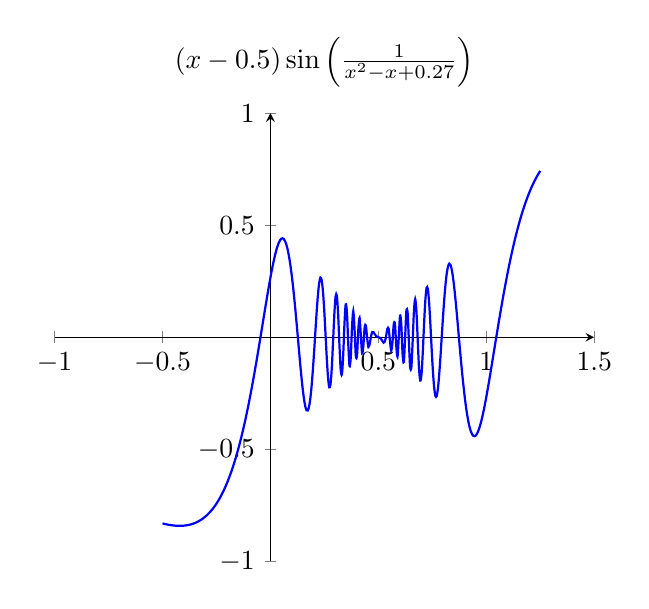
\begin{tikzpicture}[
declare function = {
f(\x) = (\x-0.5)*sin(1/(\x^2-\x+0.27));
},baseline=(current bounding box.center)]
\begin{axis}[axis lines = middle,
xmin = -1,xmax=1.5,ymin=-1,ymax=1,
trig format plots = rad,title={$(x-0.5)\sin\left(\frac{1}{x^2-x+0.27}\right)$}]
\addplot[thick,smooth,blue,domain=-0.5:1.25,samples=300]{f(x)};
\end{axis}
\end{tikzpicture}
\end{center}
\bigskip

\begin{center}
\everymath{\displaystyle}
\begin{minipage}{0.5\columnwidth}
\begin{latex}[xleftmargin=0in,
basicstyle=\color{blue!75!black}\small\tt,
]
\begin{tikzpicture}[
declare function = {
f(\x) = sin(4*\x)/cos(3*\x);
}]
\begin{axis}[axis lines = middle,
  xmin = {-7*pi/6}, xmax={7*pi/6},ymin=-5,ymax=5,
  restrict y to domain = -15:15,
  trig format plots = rad,
  title={$\frac{\sin(4x)}{\cos(3x)}$}
]
\addplot[thick,smooth,blue,
    domain={-7*pi/6}:{7*pi/6},"samples=200"]{f(x)};
\end{axis}
\end{tikzpicture}
\end{latex}
\end{minipage}
%
\tikzcount
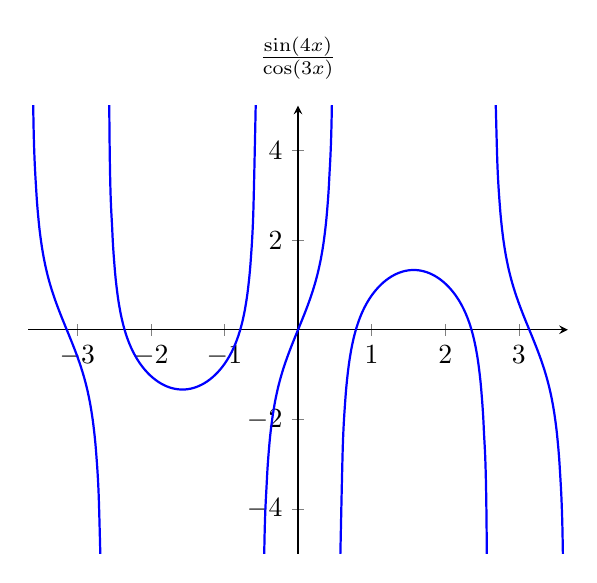
\begin{tikzpicture}[
declare function = {
f(\x) = sin(4*\x)/cos(3*\x);
},baseline=(current bounding box.center)]
\begin{axis}[axis lines = middle,
xmin = {-7*pi/6}, xmax={7*pi/6},ymin=-5,ymax=5,
restrict y to domain = -15:15,
trig format plots = rad,title={$\frac{\sin(4x)}{\cos(3x)}$}]
\addplot[thick,smooth,blue,domain={-7*pi/6}:{7*pi/6},samples=200]{f(x)};
\end{axis}
\end{tikzpicture}
\end{center}
\bigskip

\begin{center}
\begin{minipage}{0.5\columnwidth}
\begin{latex}[xleftmargin=0in,
basicstyle=\color{blue!75!black}\small\tt,
]
\begin{tikzpicture}[
declare function = {
f(\x)=tan(6*\x^2);
}]
\begin{axis}[axis lines = middle,
  xmin = {-sqrt(5*pi/12)}, xmax={sqrt(5*pi/12)},
  ymin=-5,ymax=5,
  restrict y to domain = -10:10,
  trig format plots = rad,title={$\tan(6x^2)$}]
\addplot[thick,smooth,blue,
    domain={-sqrt(5*pi/12)}:{sqrt(5*pi/12)},
    "samples=200"]{f(x)};
\end{axis}
\end{tikzpicture}
\end{latex}
\end{minipage}
%
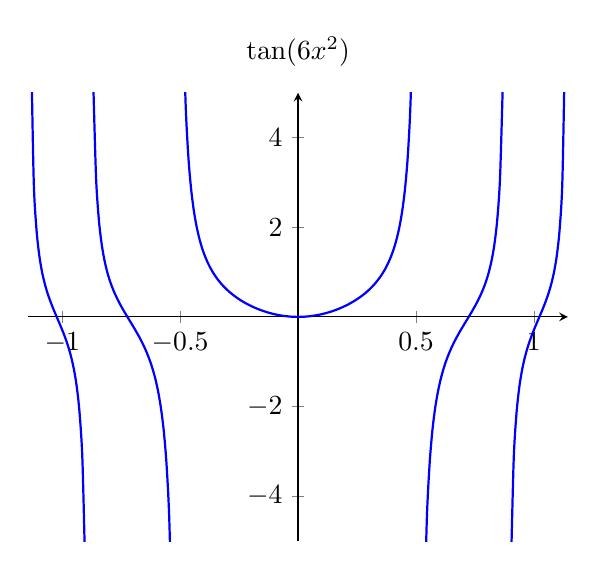
\begin{tikzpicture}[
declare function = {
f(\x)=tan(6*\x^2);
},baseline=(current bounding box.center)]
\begin{axis}[axis lines = middle,
xmin = {-sqrt(5*pi/12)}, xmax={sqrt(5*pi/12)},ymin=-5,ymax=5,
restrict y to domain = -10:10,
trig format plots = rad,title={$\tan(6x^2)$}]
\addplot[thick,smooth,blue,domain={-sqrt(5*pi/12)}:{sqrt(5*pi/12)},samples=200]{f(x)};
\end{axis}
\end{tikzpicture}
\end{center}
\bigskip

The above examples seem reasonable to me to do within "pgfplots", but
either for these, or for more extreme ones, it may be a good idea to
generate the points in an external program, such as Matlab.  Here's a
demo, followed by a more meaningful example.


We enter the following in Matlab
\begin{lstlisting}[
keepspaces=true,
basicstyle=\color{blue!75!black}\fontsize{11pt}{11pt}\tt,% scaled \tt up by 10%
columns=flexible, % prevents the extra space between letters
morekeywords={sum,linspace,fprintf},
keywordstyle=\color{red!75!black},
]
x=linspace(-3,3,10);
y=x.^2;
[x',y']
\end{lstlisting}
and then copy and paste the output into "pgfplots" as shown below
\begin{center}
\begin{minipage}{0.5\columnwidth}
\begin{latex}
\begin{tikzpicture}
\begin{axis}[axis lines = middle,enlargelimits]
\addplot[thick,blue,smooth] "table"
{ 
   -3.0000    9.0000
   -2.3333    5.4444
   -1.6667    2.7778
   -1.0000    1.0000
   -0.3333    0.1111
    0.3333    0.1111
    1.0000    1.0000
    1.6667    2.7778
    2.3333    5.4444
    3.0000    9.0000
}; % must be on line by itself
\end{axis}
\end{tikzpicture}
\end{latex}
\end{minipage}
%
\begin{tikzpicture}[baseline=(current bounding box.center)]
\begin{axis}[axis lines = middle,enlargelimits]
\addplot[thick,blue,smooth] table
{ 
   -3.0000    9.0000
   -2.3333    5.4444
   -1.6667    2.7778
   -1.0000    1.0000
   -0.3333    0.1111
    0.3333    0.1111
    1.0000    1.0000
    1.6667    2.7778
    2.3333    5.4444
    3.0000    9.0000
}; % must be on line by itself
\end{axis}
\end{tikzpicture}
\end{center}
Note that the format is quite simple: each point is defined by a pair
of numbers, on a single line with no other material, separated by a
space (or more than one spaces).

Of course for the previous example it is not necessary to use Matlab,
but for the following example I felt it was.  This is what I entered:
\begin{lstlisting}[
keepspaces=true,
basicstyle=\color{blue!75!black}\fontsize{11pt}{11pt}\tt,% scaled \tt up by 10%
columns=flexible, % prevents the extra space between letters
morekeywords={sum,linspace,fprintf},
keywordstyle=\color{red!75!black},
escapeinside=<>,
]
a=0.5;
b=5;
n=0:7;
x=linspace(-pi,pi,3000); <\color{red}\% *3000* points!>
f=@(x) (sum(a.^n.*cos(b.^n*pi.*x'), 2))';
fprintf("%g %g\n",[x; f(x)])
\end{lstlisting}
Then I copied and pasted the output into a table like above:

\begin{center}
\begin{minipage}{0.5\columnwidth}
\begin{latex}
\begin{tikzpicture}
\begin{axis}
\addplot[very thin,blue,miter limit=100] 
   table {
     -3.14159   -0.719407
     -3.1395    -0.571447
     % ...
     % most lines omitted
     % ...
     3.1395     -0.571447
     3.14159    -0.719407
   };
\end{axis}
\end{tikzpicture}
\end{latex}
\end{minipage}
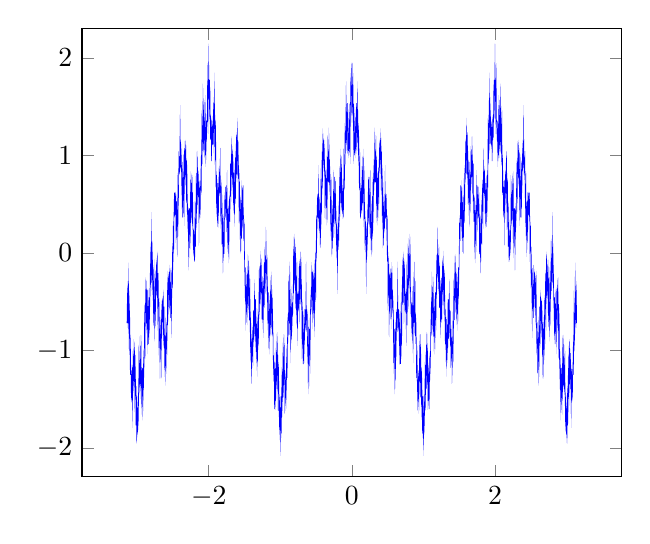
\begin{tikzpicture}[baseline=(current bounding box.center)]
\begin{axis}
\addplot[very thin,blue,miter limit=100] 
table {
-3.14159 -0.719407
-3.1395 -0.571447
-3.1374 -0.503857
-3.13531 -0.402893
-3.13321 -0.447329
-3.13112 -0.637915
-3.12902 -0.594599
-3.12693 -0.565763
-3.12483 -0.63422
-3.12274 -0.419754
-3.12064 -0.325949
-3.11855 -0.506732
-3.11645 -0.5339
-3.11436 -0.649685
-3.11226 -0.807189
-3.11017 -0.728248
-3.10807 -0.75086
-3.10598 -0.727093
-3.10388 -0.634305
-3.10179 -0.884654
-3.09969 -1.02556
-3.0976 -1.00759
-3.0955 -1.24539
-3.09341 -1.24463
-3.09131 -1.06861
-3.08922 -1.16524
-3.08712 -1.18364
-3.08503 -1.22203
-3.08293 -1.42409
-3.08083 -1.44787
-3.07874 -1.48381
-3.07664 -1.49505
-3.07455 -1.27092
-3.07245 -1.25122
-3.07036 -1.35989
-3.06826 -1.29392
-3.06617 -1.39343
-3.06407 -1.52853
-3.06198 -1.37444
-3.05988 -1.23672
-3.05779 -1.1811
-3.05569 -1.08226
-3.0536 -1.12107
-3.0515 -1.21657
-3.04941 -1.24109
-3.04731 -1.3026
-3.04522 -1.21599
-3.04312 -1.01601
-3.04103 -1.05949
-3.03893 -1.09688
-3.03684 -1.05005
-3.03474 -1.27441
-3.03265 -1.40337
-3.03055 -1.28493
-3.02846 -1.32089
-3.02636 -1.2922
-3.02427 -1.2219
-3.02217 -1.37697
-3.02008 -1.44574
-3.01798 -1.56438
-3.01589 -1.7673
-3.01379 -1.63252
-3.0117 -1.58265
-3.0096 -1.69141
-3.00751 -1.53341
-3.00541 -1.59863
-3.00332 -1.85357
-3.00122 -1.82286
-2.99913 -1.84992
-2.99703 -1.84103
-2.99494 -1.63872
-2.99284 -1.61657
-2.99075 -1.57699
-2.98865 -1.54222
-2.98656 -1.7475
-2.98446 -1.72058
-2.98237 -1.54017
-2.98027 -1.54617
-2.97818 -1.37927
-2.97608 -1.1836
-2.97399 -1.28122
-2.97189 -1.34119
-2.96979 -1.32969
-2.9677 -1.36157
-2.9656 -1.25752
-2.96351 -1.13613
-2.96141 -1.08524
-2.95932 -0.992769
-2.95722 -1.06774
-2.95513 -1.25256
-2.95303 -1.21677
-2.95094 -1.21315
-2.94884 -1.29535
-2.94675 -1.12612
-2.94465 -1.04407
-2.94256 -1.20138
-2.94046 -1.23494
-2.93837 -1.33472
-2.93627 -1.47885
-2.93418 -1.40641
-2.93208 -1.39658
-2.92999 -1.33096
-2.92789 -1.17697
-2.9258 -1.35394
-2.9237 -1.4581
-2.92161 -1.37978
-2.91951 -1.54293
-2.91742 -1.47754
-2.91532 -1.19564
-2.91323 -1.19606
-2.91113 -1.14092
-2.90904 -1.10068
-2.90694 -1.24376
-2.90485 -1.18009
-2.90275 -1.12077
-2.90066 -1.07177
-2.89856 -0.769888
-2.89647 -0.703016
-2.89437 -0.795328
-2.89228 -0.67566
-2.89018 -0.736564
-2.88809 -0.839181
-2.88599 -0.65626
-2.8839 -0.538093
-2.8818 -0.48441
-2.87971 -0.388839
-2.87761 -0.451399
-2.87552 -0.526239
-2.87342 -0.560018
-2.87133 -0.666737
-2.86923 -0.596569
-2.86714 -0.429001
-2.86504 -0.484002
-2.86295 -0.507515
-2.86085 -0.474714
-2.85876 -0.692913
-2.85666 -0.829024
-2.85456 -0.732455
-2.85247 -0.7286
-2.85037 -0.662195
-2.84828 -0.562651
-2.84618 -0.665582
-2.84409 -0.709884
-2.84199 -0.791042
-2.8399 -0.935384
-2.8378 -0.743515
-2.83571 -0.604199
-2.83361 -0.651076
-2.83152 -0.456867
-2.82942 -0.456762
-2.82733 -0.663788
-2.82523 -0.57626
-2.82314 -0.529571
-2.82104 -0.480995
-2.81895 -0.244008
-2.81685 -0.210839
-2.81476 -0.169259
-2.81266 -0.0965404
-2.81057 -0.295958
-2.80847 -0.277154
-2.80638 -0.0988365
-2.80428 -0.156969
-2.80219 -0.0321146
-2.80009 0.137693
-2.798 -0.00129609
-2.7959 -0.0849199
-2.79381 -0.135103
-2.79171 -0.24617
-2.78962 -0.186662
-2.78752 -0.135741
-2.78543 -0.131318
-2.78333 -0.0538376
-2.78124 -0.189835
-2.77914 -0.4251
-2.77705 -0.431657
-2.77495 -0.473265
-2.77286 -0.551907
-2.77076 -0.391808
-2.76867 -0.321445
-2.76657 -0.466133
-2.76448 -0.526184
-2.76238 -0.625636
-2.76029 -0.727423
-2.75819 -0.635577
-2.7561 -0.591271
-2.754 -0.503242
-2.75191 -0.346856
-2.74981 -0.494754
-2.74772 -0.582564
-2.74562 -0.472953
-2.74352 -0.592626
-2.74143 -0.53851
-2.73933 -0.265826
-2.73724 -0.269685
-2.73514 -0.236187
-2.73305 -0.19494
-2.73095 -0.356076
-2.72886 -0.330484
-2.72676 -0.315754
-2.72467 -0.349364
-2.72257 -0.102231
-2.72048 -0.0743944
-2.71838 -0.24151
-2.71629 -0.181925
-2.71419 -0.324114
-2.7121 -0.530648
-2.71 -0.419761
-2.70791 -0.379207
-2.70581 -0.381935
-2.70372 -0.335304
-2.70162 -0.492338
-2.69953 -0.629843
-2.69743 -0.713281
-2.69534 -0.882488
-2.69324 -0.820652
-2.69115 -0.669802
-2.68905 -0.760439
-2.68696 -0.796539
-2.68486 -0.791976
-2.68277 -1.00147
-2.68067 -1.10241
-2.67858 -1.00288
-2.67648 -0.967956
-2.67439 -0.88307
-2.67229 -0.793969
-2.6702 -0.858496
-2.6681 -0.865738
-2.66601 -0.918838
-2.66391 -1.03009
-2.66182 -0.84592
-2.65972 -0.703509
-2.65763 -0.742164
-2.65553 -0.559049
-2.65344 -0.537023
-2.65134 -0.749376
-2.64925 -0.708553
-2.64715 -0.693973
-2.64506 -0.692787
-2.64296 -0.492104
-2.64087 -0.48464
-2.63877 -0.496621
-2.63668 -0.469069
-2.63458 -0.739334
-2.63248 -0.804473
-2.63039 -0.660017
-2.62829 -0.762444
-2.6262 -0.685869
-2.6241 -0.550091
-2.62201 -0.751936
-2.61991 -0.876068
-2.61782 -0.950448
-2.61572 -1.08225
-2.61363 -0.998831
-2.61153 -0.95261
-2.60944 -0.96659
-2.60734 -0.862286
-2.60525 -0.986124
-2.60315 -1.18408
-2.60106 -1.12098
-2.59896 -1.12393
-2.59687 -1.1507
-2.59477 -0.948425
-2.59268 -0.84152
-2.59058 -0.895712
-2.58849 -0.888567
-2.58639 -0.934691
-2.5843 -0.962676
-2.5822 -0.844647
-2.58011 -0.766833
-2.57801 -0.618729
-2.57592 -0.42234
-2.57382 -0.518834
-2.57173 -0.587919
-2.56963 -0.487867
-2.56754 -0.5908
-2.56544 -0.544637
-2.56335 -0.27129
-2.56125 -0.25175
-2.55916 -0.241866
-2.55706 -0.230038
-2.55497 -0.418561
-2.55287 -0.424638
-2.55078 -0.408636
-2.54868 -0.456188
-2.54659 -0.225637
-2.54449 -0.201581
-2.5424 -0.407177
-2.5403 -0.355962
-2.53821 -0.471288
-2.53611 -0.664379
-2.53402 -0.519729
-2.53192 -0.45895
-2.52983 -0.445663
-2.52773 -0.347985
-2.52564 -0.463324
-2.52354 -0.525564
-2.52144 -0.514091
-2.51935 -0.637821
-2.51725 -0.508935
-2.51516 -0.279228
-2.51306 -0.302807
-2.51097 -0.231695
-2.50887 -0.137737
-2.50678 -0.273512
-2.50468 -0.294429
-2.50259 -0.157279
-2.50049 -0.0552288
-2.4984 0.119252
-2.4963 0.251501
-2.49421 0.243346
-2.49211 0.271924
-2.49002 0.216426
-2.48792 0.130742
-2.48583 0.329535
-2.48373 0.488412
-2.48164 0.468916
-2.47954 0.617241
-2.47745 0.61746
-2.47535 0.393351
-2.47326 0.399483
-2.47116 0.416167
-2.46907 0.410515
-2.46697 0.576361
-2.46488 0.560596
-2.46278 0.514877
-2.46069 0.539501
-2.45859 0.28702
-2.4565 0.216323
-2.4544 0.379635
-2.45231 0.284497
-2.45021 0.353256
-2.44812 0.529862
-2.44602 0.373998
-2.44393 0.302143
-2.44183 0.285287
-2.43974 0.17976
-2.43764 0.315331
-2.43555 0.418694
-2.43345 0.453156
-2.43136 0.650687
-2.42926 0.58967
-2.42717 0.422261
-2.42507 0.536936
-2.42298 0.562967
-2.42088 0.581975
-2.41879 0.83989
-2.41669 0.962623
-2.4146 0.934992
-2.4125 0.936087
-2.41041 0.855537
-2.40831 0.84184
-2.40621 0.950172
-2.40412 0.996561
-2.40202 1.12432
-2.39993 1.25536
-2.39783 1.10005
-2.39574 0.985561
-2.39364 1.02588
-2.39155 0.894403
-2.38945 0.881759
-2.38736 1.06686
-2.38526 1.0368
-2.38317 0.984947
-2.38107 0.948184
-2.37898 0.742994
-2.37688 0.694525
-2.37479 0.673577
-2.37269 0.586237
-2.3706 0.780405
-2.3685 0.819006
-2.36641 0.616887
-2.36431 0.667678
-2.36222 0.572041
-2.36012 0.366439
-2.35803 0.51514
-2.35593 0.607252
-2.35384 0.647446
-2.35174 0.789242
-2.34965 0.685245
-2.34755 0.619863
-2.34546 0.655223
-2.34336 0.527767
-2.34127 0.670485
-2.33917 0.930573
-2.33708 0.884432
-2.33498 0.93195
-2.33289 0.992829
-2.33079 0.811324
-2.3287 0.777
-2.3266 0.868059
-2.32451 0.911346
-2.32241 1.0364
-2.32032 1.06575
-2.31822 0.976897
-2.31613 0.955214
-2.31403 0.816728
-2.31194 0.662973
-2.30984 0.775742
-2.30775 0.828795
-2.30565 0.739547
-2.30356 0.807308
-2.30146 0.749957
-2.29937 0.49468
-2.29727 0.421312
-2.29517 0.375637
-2.29308 0.332634
-2.29098 0.453613
-2.28889 0.434655
-2.28679 0.385491
-2.2847 0.396722
-2.2826 0.14329
-2.28051 0.0489917
-2.27841 0.223395
-2.27632 0.169854
-2.27422 0.252314
-2.27213 0.458578
-2.27003 0.320478
-2.26794 0.243851
-2.26584 0.248733
-2.26375 0.160043
-2.26165 0.323477
-2.25956 0.450273
-2.25746 0.45778
-2.25537 0.645301
-2.25327 0.57313
-2.25118 0.372229
-2.24908 0.487268
-2.24699 0.488897
-2.24489 0.454077
-2.2428 0.663188
-2.2407 0.710718
-2.23861 0.638091
-2.23651 0.605922
-2.23442 0.453578
-2.23232 0.393425
-2.23023 0.434973
-2.22813 0.38913
-2.22604 0.478851
-2.22394 0.570679
-2.22185 0.378041
-2.21975 0.241504
-2.21766 0.225398
-2.21556 0.0661124
-2.21347 0.0452711
-2.21137 0.21365
-2.20928 0.220659
-2.20718 0.193138
-2.20509 0.151419
-2.20299 -0.02344
-2.2009 -0.0458332
-2.1988 -0.0207331
-2.19671 -0.0363456
-2.19461 0.20557
-2.19252 0.305031
-2.19042 0.14762
-2.18833 0.226612
-2.18623 0.207139
-2.18413 0.0665214
-2.18204 0.262849
-2.17994 0.408775
-2.17785 0.467324
-2.17575 0.632508
-2.17366 0.557298
-2.17156 0.511212
-2.16947 0.588161
-2.16737 0.4606
-2.16528 0.57523
-2.16318 0.833201
-2.16109 0.761807
-2.15899 0.797311
-2.1569 0.863009
-2.1548 0.651031
-2.15271 0.591847
-2.15061 0.640958
-2.14852 0.64094
-2.14642 0.776179
-2.14433 0.793288
-2.14223 0.68955
-2.14014 0.678941
-2.13804 0.512573
-2.13595 0.355506
-2.13385 0.500905
-2.13176 0.579513
-2.12966 0.546739
-2.12757 0.649171
-2.12547 0.613927
-2.12338 0.426075
-2.12128 0.403182
-2.11919 0.428649
-2.11709 0.492
-2.115 0.674362
-2.1129 0.719753
-2.11081 0.743668
-2.10871 0.819088
-2.10662 0.663902
-2.10452 0.64815
-2.10243 0.885039
-2.10033 0.902162
-2.09824 1.01011
-2.09614 1.2551
-2.09405 1.18214
-2.09195 1.13973
-2.08986 1.17824
-2.08776 1.09843
-2.08567 1.24793
-2.08357 1.37836
-2.08148 1.37181
-2.07938 1.56204
-2.07729 1.49928
-2.07519 1.25402
-2.07309 1.33474
-2.071 1.30941
-2.0689 1.2384
-2.06681 1.44684
-2.06471 1.47997
-2.06262 1.38669
-2.06052 1.3433
-2.05843 1.14976
-2.05633 1.09221
-2.05424 1.16604
-2.05214 1.12255
-2.05005 1.24436
-2.04795 1.35847
-2.04586 1.16967
-2.04376 1.0805
-2.04167 1.10891
-2.03957 1.01134
-2.03748 1.06403
-2.03538 1.25616
-2.03329 1.31202
-2.03119 1.34672
-2.0291 1.3422
-2.027 1.24461
-2.02491 1.28293
-2.02281 1.33123
-2.02072 1.34761
-2.01862 1.59749
-2.01653 1.72261
-2.01443 1.60303
-2.01234 1.67633
-2.01024 1.65937
-2.00815 1.49843
-2.00605 1.63853
-2.00396 1.76343
-2.00186 1.79589
-1.99977 1.92271
-1.99767 1.80597
-1.99558 1.68089
-1.99348 1.69254
-1.99139 1.50408
-1.98929 1.54819
-1.9872 1.77547
-1.9851 1.65094
-1.98301 1.60747
-1.98091 1.61966
-1.97882 1.34736
-1.97672 1.25507
-1.97463 1.28988
-1.97253 1.25512
-1.97044 1.3798
-1.96834 1.36796
-1.96625 1.229
-1.96415 1.24419
-1.96206 1.09157
-1.95996 0.943463
-1.95786 1.11579
-1.95577 1.18565
-1.95367 1.16366
-1.95158 1.29151
-1.94948 1.27021
-1.94739 1.13077
-1.94529 1.11756
-1.9432 1.11945
-1.9411 1.19426
-1.93901 1.36173
-1.93691 1.39698
-1.93482 1.43215
-1.93272 1.47342
-1.93063 1.27842
-1.92853 1.20641
-1.92644 1.37033
-1.92434 1.35547
-1.92225 1.40658
-1.92015 1.57382
-1.91806 1.43832
-1.91596 1.29175
-1.91387 1.23261
-1.91177 1.08365
-1.90968 1.15451
-1.90758 1.22129
-1.90549 1.12781
-1.90339 1.21983
-1.9013 1.09392
-1.8992 0.773889
-1.89711 0.804295
-1.89501 0.758044
-1.89292 0.632419
-1.89082 0.796484
-1.88873 0.794545
-1.88663 0.674446
-1.88454 0.646938
-1.88244 0.45311
-1.88035 0.398037
-1.87825 0.490278
-1.87616 0.425881
-1.87406 0.559449
-1.87197 0.716891
-1.86987 0.545769
-1.86778 0.489735
-1.86568 0.526439
-1.86359 0.417613
-1.86149 0.488027
-1.8594 0.674282
-1.8573 0.74135
-1.85521 0.799477
-1.85311 0.753237
-1.85102 0.622106
-1.84892 0.634409
-1.84682 0.631591
-1.84473 0.628664
-1.84263 0.841076
-1.84054 0.905162
-1.83844 0.731883
-1.83635 0.715821
-1.83425 0.63718
-1.83216 0.444202
-1.83006 0.515761
-1.82797 0.589238
-1.82587 0.565589
-1.82378 0.614559
-1.82168 0.457622
-1.81959 0.299763
-1.81749 0.294627
-1.8154 0.101036
-1.8133 0.105296
-1.81121 0.320414
-1.80911 0.20419
-1.80702 0.163055
-1.80492 0.221899
-1.80283 -0.00936579
-1.80073 -0.0785128
-1.79864 -0.00731741
-1.79654 -0.016096
-1.79445 0.170597
-1.79235 0.235507
-1.79026 0.142939
-1.78816 0.226646
-1.78607 0.118668
-1.78397 -0.00974603
-1.78188 0.225122
-1.77978 0.346382
-1.77769 0.370688
-1.77559 0.542575
-1.7735 0.517954
-1.7714 0.393047
-1.76931 0.393227
-1.76721 0.385203
-1.76512 0.490592
-1.76302 0.655547
-1.76093 0.648606
-1.75883 0.667967
-1.75674 0.674277
-1.75464 0.459414
-1.75255 0.387276
-1.75045 0.517445
-1.74836 0.485286
-1.74626 0.505257
-1.74417 0.625432
-1.74207 0.502995
-1.73998 0.365141
-1.73788 0.30314
-1.73578 0.17459
-1.73369 0.241368
-1.73159 0.321575
-1.7295 0.268294
-1.7274 0.402471
-1.72531 0.354034
-1.72321 0.0887575
-1.72112 0.153934
-1.71902 0.180056
-1.71693 0.118223
-1.71483 0.361509
-1.71274 0.462094
-1.71064 0.415745
-1.70855 0.462539
-1.70645 0.326504
-1.70436 0.325584
-1.70226 0.512212
-1.70017 0.513161
-1.69807 0.699033
-1.69598 0.916905
-1.69388 0.757891
-1.69179 0.723751
-1.68969 0.797293
-1.6876 0.705667
-1.6855 0.806303
-1.68341 0.981675
-1.68131 1.01692
-1.67922 1.07493
-1.67712 0.998028
-1.67503 0.852481
-1.67293 0.874838
-1.67084 0.829925
-1.66874 0.791386
-1.66665 0.974882
-1.66455 1.00436
-1.66246 0.841442
-1.66036 0.819016
-1.65827 0.727379
-1.65617 0.545523
-1.65408 0.591316
-1.65198 0.668313
-1.64989 0.693444
-1.64779 0.769733
-1.6457 0.65683
-1.6436 0.535155
-1.64151 0.551149
-1.63941 0.411974
-1.63732 0.464232
-1.63522 0.746462
-1.63313 0.714519
-1.63103 0.707724
-1.62894 0.807854
-1.62684 0.62946
-1.62474 0.59816
-1.62265 0.731519
-1.62055 0.767207
-1.61846 0.978662
-1.61636 1.06347
-1.61427 0.953505
-1.61217 1.04535
-1.61008 0.957601
-1.60798 0.807596
-1.60589 1.02973
-1.60379 1.11353
-1.6017 1.07349
-1.5996 1.20803
-1.59751 1.1335
-1.59541 0.970093
-1.59332 0.930913
-1.59122 0.831191
-1.58913 0.871599
-1.58703 0.981487
-1.58494 0.901479
-1.58284 0.895752
-1.58075 0.863278
-1.57865 0.586054
-1.57656 0.473525
-1.57446 0.548373
-1.57237 0.498049
-1.57027 0.527275
-1.56818 0.624598
-1.56608 0.508562
-1.56399 0.36858
-1.56189 0.279524
-1.5598 0.177374
-1.5577 0.273538
-1.55561 0.376991
-1.55351 0.356582
-1.55142 0.487967
-1.54932 0.452253
-1.54723 0.209488
-1.54513 0.279378
-1.54304 0.343632
-1.54094 0.29398
-1.53885 0.508907
-1.53675 0.597637
-1.53466 0.524534
-1.53256 0.552218
-1.53047 0.402976
-1.52837 0.354887
-1.52628 0.497532
-1.52418 0.425949
-1.52209 0.521825
-1.51999 0.694039
-1.5179 0.471303
-1.5158 0.359569
-1.51371 0.362079
-1.51161 0.164781
-1.50951 0.177148
-1.50742 0.276755
-1.50532 0.23383
-1.50323 0.252094
-1.50113 0.102467
-1.49904 -0.133005
-1.49694 -0.155862
-1.49485 -0.260106
-1.49275 -0.333356
-1.49066 -0.151421
-1.48856 -0.153242
-1.48647 -0.331481
-1.48437 -0.373644
-1.48228 -0.486263
-1.48018 -0.630829
-1.47809 -0.566618
-1.47599 -0.48119
-1.4739 -0.420643
-1.4718 -0.34936
-1.46971 -0.454199
-1.46761 -0.536304
-1.46552 -0.498789
-1.46342 -0.6035
-1.46133 -0.546109
-1.45923 -0.283882
-1.45714 -0.305981
-1.45504 -0.326344
-1.45295 -0.234031
-1.45085 -0.40092
-1.44876 -0.471554
-1.44666 -0.38625
-1.44457 -0.397643
-1.44247 -0.240796
-1.44038 -0.182768
-1.43828 -0.34118
-1.43619 -0.308206
-1.43409 -0.447244
-1.432 -0.687014
-1.4299 -0.528574
-1.42781 -0.476535
-1.42571 -0.566621
-1.42362 -0.466315
-1.42152 -0.590496
-1.41943 -0.808972
-1.41733 -0.867557
-1.41524 -0.995059
-1.41314 -0.94885
-1.41105 -0.811197
-1.40895 -0.909179
-1.40686 -0.906252
-1.40476 -0.911326
-1.40267 -1.16776
-1.40057 -1.21467
-1.39847 -1.08635
-1.39638 -1.09273
-1.39428 -1.00429
-1.39219 -0.881027
-1.39009 -0.934858
-1.388 -0.98455
-1.3859 -1.02656
-1.38381 -1.06504
-1.38171 -0.919909
-1.37962 -0.800459
-1.37752 -0.772369
-1.37543 -0.601486
-1.37333 -0.597707
-1.37124 -0.799978
-1.36914 -0.745099
-1.36705 -0.683937
-1.36495 -0.726665
-1.36286 -0.530674
-1.36076 -0.428881
-1.35867 -0.502908
-1.35657 -0.509924
-1.35448 -0.685861
-1.35238 -0.774115
-1.35029 -0.644971
-1.34819 -0.712887
-1.3461 -0.640977
-1.344 -0.47144
-1.34191 -0.708682
-1.33981 -0.850504
-1.33772 -0.829282
-1.33562 -1.00234
-1.33353 -0.959532
-1.33143 -0.821229
-1.32934 -0.851717
-1.32724 -0.789345
-1.32515 -0.883226
-1.32305 -1.06734
-1.32096 -0.989989
-1.31886 -1.01831
-1.31677 -1.04087
-1.31467 -0.777747
-1.31258 -0.71192
-1.31048 -0.799855
-1.30839 -0.737065
-1.30629 -0.781235
-1.3042 -0.842546
-1.3021 -0.721318
-1.30001 -0.602338
-1.29791 -0.45612
-1.29582 -0.322128
-1.29372 -0.388181
-1.29163 -0.421807
-1.28953 -0.381846
-1.28743 -0.479137
-1.28534 -0.402429
-1.28324 -0.139707
-1.28115 -0.135854
-1.27905 -0.165607
-1.27696 -0.117774
-1.27486 -0.294712
-1.27277 -0.392008
-1.27067 -0.326613
-1.26858 -0.331341
-1.26648 -0.198457
-1.26439 -0.162326
-1.26229 -0.346439
-1.2602 -0.337875
-1.2581 -0.452662
-1.25601 -0.681067
-1.25391 -0.516692
-1.25182 -0.436258
-1.24972 -0.525753
-1.24763 -0.404181
-1.24553 -0.475578
-1.24344 -0.64361
-1.24134 -0.632143
-1.23925 -0.717123
-1.23715 -0.636564
-1.23506 -0.429506
-1.23296 -0.478795
-1.23087 -0.406163
-1.22877 -0.32185
-1.22668 -0.539193
-1.22458 -0.544693
-1.22249 -0.379344
-1.22039 -0.358423
-1.2183 -0.209407
-1.2162 -0.0590129
-1.21411 -0.101405
-1.21201 -0.13212
-1.20992 -0.210553
-1.20782 -0.266873
-1.20573 -0.113189
-1.20363 -0.0243999
-1.20154 -0.0190694
-1.19944 0.105567
-1.19735 0.0370339
-1.19525 -0.207464
-1.19316 -0.212632
-1.19106 -0.197374
-1.18897 -0.266505
-1.18687 -0.150796
-1.18478 -0.116281
-1.18268 -0.234912
-1.18059 -0.298329
-1.17849 -0.493848
-1.17639 -0.605494
-1.1743 -0.511987
-1.1722 -0.601362
-1.17011 -0.570258
-1.16801 -0.404655
-1.16592 -0.6132
-1.16382 -0.753668
-1.16173 -0.713542
-1.15963 -0.874508
-1.15754 -0.83641
-1.15544 -0.669874
-1.15335 -0.6719
-1.15125 -0.567824
-1.14916 -0.621649
-1.14706 -0.813154
-1.14497 -0.722974
-1.14287 -0.735349
-1.14078 -0.762833
-1.13868 -0.471124
-1.13659 -0.402294
-1.13449 -0.518921
-1.1324 -0.481134
-1.1303 -0.578847
-1.12821 -0.6682
-1.12611 -0.568482
-1.12402 -0.516279
-1.12192 -0.417855
-1.11983 -0.356475
-1.11773 -0.526574
-1.11564 -0.616863
-1.11354 -0.642627
-1.11145 -0.812953
-1.10935 -0.800461
-1.10726 -0.640766
-1.10516 -0.714845
-1.10307 -0.805515
-1.10097 -0.832117
-1.09888 -1.03492
-1.09678 -1.17366
-1.09469 -1.18013
-1.09259 -1.21892
-1.0905 -1.12077
-1.0884 -1.09758
-1.08631 -1.26697
-1.08421 -1.26619
-1.08212 -1.37247
-1.08002 -1.60199
-1.07793 -1.44888
-1.07583 -1.32536
-1.07374 -1.37752
-1.07164 -1.23266
-1.06955 -1.2699
-1.06745 -1.43405
-1.06536 -1.40909
-1.06326 -1.47053
-1.06116 -1.37408
-1.05907 -1.12806
-1.05697 -1.17868
-1.05488 -1.13514
-1.05278 -1.05339
-1.05069 -1.29748
-1.04859 -1.3208
-1.0465 -1.16075
-1.0444 -1.18506
-1.04231 -1.07949
-1.04021 -0.991979
-1.03812 -1.10327
-1.03602 -1.1556
-1.03393 -1.28509
-1.03183 -1.40272
-1.02974 -1.28855
-1.02764 -1.28035
-1.02555 -1.33327
-1.02345 -1.23296
-1.02136 -1.33702
-1.01926 -1.58991
-1.01717 -1.62597
-1.01507 -1.65309
-1.01298 -1.71533
-1.01088 -1.60539
-1.00879 -1.55364
-1.00669 -1.6165
-1.0046 -1.66526
-1.0025 -1.8377
-1.00041 -1.90935
-0.998312 -1.77747
-0.996217 -1.7876
-0.994122 -1.69039
-0.992027 -1.46927
-0.989932 -1.6068
-0.987837 -1.71408
-0.985741 -1.62197
-0.983646 -1.69942
-0.981551 -1.60591
-0.979456 -1.38207
-0.977361 -1.34766
-0.975266 -1.22734
-0.973171 -1.24554
-0.971076 -1.41969
-0.968981 -1.29917
-0.966886 -1.27751
-0.964791 -1.32727
-0.962695 -1.04971
-0.9606 -0.988734
-0.958505 -1.12665
-0.95641 -1.08081
-0.954315 -1.19046
-0.95222 -1.30402
-0.950125 -1.2217
-0.94803 -1.21808
-0.945935 -1.12671
-0.94384 -1.04496
-0.941745 -1.22846
-0.939649 -1.30531
-0.937554 -1.32676
-0.935459 -1.50936
-0.933364 -1.46211
-0.931269 -1.26696
-0.929174 -1.28626
-0.927079 -1.30644
-0.924984 -1.30729
-0.922889 -1.4531
-0.920794 -1.51353
-0.918698 -1.46041
-0.916603 -1.39366
-0.914508 -1.19972
-0.912413 -1.11175
-0.910318 -1.19955
-0.908223 -1.13389
-0.906128 -1.153
-0.904033 -1.2792
-0.901938 -1.06381
-0.899843 -0.866897
-0.897748 -0.863802
-0.895652 -0.697019
-0.893557 -0.676418
-0.891462 -0.789588
-0.889367 -0.730531
-0.887272 -0.764188
-0.885177 -0.679595
-0.883082 -0.433944
-0.880987 -0.482819
-0.878892 -0.453035
-0.876797 -0.352785
-0.874702 -0.607497
-0.872606 -0.673469
-0.870511 -0.533982
-0.868416 -0.588301
-0.866321 -0.489954
-0.864226 -0.395098
-0.862131 -0.5243
-0.860036 -0.573677
-0.857941 -0.718614
-0.855846 -0.857836
-0.853751 -0.70328
-0.851655 -0.665446
-0.84956 -0.692967
-0.847465 -0.546118
-0.84537 -0.634752
-0.843275 -0.84799
-0.84118 -0.824275
-0.839085 -0.799349
-0.83699 -0.771091
-0.834895 -0.603407
-0.8328 -0.521204
-0.830705 -0.511658
-0.828609 -0.508926
-0.826514 -0.623089
-0.824419 -0.61318
-0.822324 -0.443614
-0.820229 -0.419376
-0.818134 -0.300497
-0.816039 -0.0734987
-0.813944 -0.165791
-0.811849 -0.256484
-0.809754 -0.174596
-0.807659 -0.250854
-0.805563 -0.200678
-0.803468 -0.0176395
-0.801373 -0.00019961
-0.799278 0.085693
-0.797183 0.0390456
-0.795088 -0.194205
-0.792993 -0.151037
-0.790898 -0.176658
-0.788803 -0.290312
-0.786708 -0.0591993
-0.784613 -0.0211849
-0.782517 -0.221157
-0.780422 -0.231133
-0.778327 -0.388601
-0.776232 -0.54373
-0.774137 -0.461929
-0.772042 -0.475603
-0.769947 -0.399016
-0.767852 -0.313228
-0.765757 -0.528069
-0.763662 -0.600665
-0.761566 -0.582995
-0.759471 -0.750066
-0.757376 -0.66877
-0.755281 -0.458462
-0.753186 -0.476262
-0.751091 -0.460039
-0.748996 -0.444263
-0.746901 -0.555761
-0.744806 -0.568342
-0.742711 -0.530716
-0.740616 -0.468774
-0.73852 -0.268739
-0.736425 -0.199865
-0.73433 -0.277798
-0.732235 -0.224534
-0.73014 -0.28492
-0.728045 -0.448288
-0.72595 -0.308662
-0.723855 -0.164666
-0.72176 -0.190493
-0.719665 -0.097334
-0.71757 -0.141744
-0.715474 -0.330951
-0.713379 -0.376142
-0.711284 -0.482102
-0.709189 -0.468391
-0.707094 -0.285009
-0.704999 -0.389861
-0.702904 -0.454957
-0.700809 -0.425039
-0.698714 -0.730952
-0.696619 -0.856813
-0.694523 -0.73519
-0.692428 -0.813007
-0.690333 -0.75489
-0.688238 -0.682888
-0.686143 -0.840756
-0.684048 -0.880001
-0.681953 -0.997003
-0.679858 -1.13595
-0.677763 -0.954461
-0.675668 -0.905755
-0.673573 -0.940236
-0.671477 -0.751305
-0.669382 -0.80476
-0.667287 -0.986374
-0.665192 -0.93028
-0.663097 -0.916297
-0.661002 -0.876949
-0.658907 -0.695105
-0.656812 -0.621586
-0.654717 -0.582056
-0.652622 -0.584411
-0.650527 -0.746162
-0.648431 -0.758805
-0.646336 -0.632646
-0.644241 -0.641004
-0.642146 -0.539815
-0.640051 -0.370399
-0.637956 -0.509737
-0.635861 -0.665334
-0.633766 -0.669431
-0.631671 -0.7768
-0.629576 -0.767367
-0.62748 -0.642625
-0.625385 -0.663332
-0.62329 -0.641688
-0.621195 -0.736597
-0.6191 -0.992091
-0.617005 -0.971442
-0.61491 -0.985456
-0.612815 -1.10818
-0.61072 -0.902597
-0.608625 -0.84658
-0.60653 -1.03146
-0.604434 -1.00766
-0.602339 -1.10404
-0.600244 -1.22213
-0.598149 -1.09587
-0.596054 -1.07183
-0.593959 -0.952857
-0.591864 -0.777585
-0.589769 -0.926678
-0.587674 -0.94319
-0.585579 -0.855887
-0.583484 -0.99532
-0.581388 -0.871265
-0.579293 -0.598508
-0.577198 -0.572106
-0.575103 -0.498874
-0.573008 -0.466817
-0.570913 -0.583542
-0.568818 -0.569669
-0.566723 -0.537384
-0.564628 -0.468634
-0.562533 -0.241118
-0.560438 -0.201076
-0.558342 -0.305306
-0.556247 -0.27439
-0.554152 -0.367619
-0.552057 -0.52439
-0.549962 -0.39991
-0.547867 -0.28243
-0.545772 -0.312137
-0.543677 -0.260143
-0.541582 -0.317944
-0.539487 -0.476535
-0.537391 -0.514923
-0.535296 -0.598125
-0.533201 -0.566322
-0.531106 -0.375395
-0.529011 -0.433531
-0.526916 -0.453331
-0.524821 -0.35631
-0.522726 -0.573708
-0.520631 -0.655341
-0.518536 -0.475059
-0.516441 -0.47291
-0.514345 -0.342243
-0.51225 -0.167467
-0.510155 -0.234987
-0.50806 -0.199394
-0.505965 -0.240289
-0.50387 -0.334151
-0.501775 -0.0777066
-0.49968 0.0616191
-0.497585 0.0768552
-0.49549 0.324416
-0.493395 0.306009
-0.491299 0.132098
-0.489204 0.221649
-0.487109 0.253704
-0.485014 0.317276
-0.482919 0.518383
-0.480824 0.554976
-0.478729 0.580205
-0.476634 0.569643
-0.474539 0.37499
-0.472444 0.36992
-0.470348 0.484025
-0.468253 0.435052
-0.466158 0.515548
-0.464063 0.647716
-0.461968 0.5047
-0.459873 0.369366
-0.457778 0.349571
-0.455683 0.25417
-0.453588 0.269604
-0.451493 0.378529
-0.449398 0.398976
-0.447302 0.467495
-0.445207 0.414319
-0.443112 0.213406
-0.441017 0.258004
-0.438922 0.289659
-0.436827 0.229909
-0.434732 0.485762
-0.432637 0.629417
-0.430542 0.510681
-0.428447 0.563805
-0.426352 0.518307
-0.424256 0.440689
-0.422161 0.616879
-0.420066 0.698075
-0.417971 0.840082
-0.415876 1.04123
-0.413781 0.890014
-0.411686 0.851878
-0.409591 0.9582
-0.407496 0.814647
-0.405401 0.913891
-0.403305 1.16353
-0.40121 1.12791
-0.399115 1.15109
-0.39702 1.13948
-0.394925 0.967593
-0.39283 0.955396
-0.390735 0.921775
-0.38864 0.901707
-0.386545 1.08177
-0.38445 1.05666
-0.382355 0.905831
-0.380259 0.917824
-0.378164 0.7712
-0.376069 0.574763
-0.373974 0.656602
-0.371879 0.73145
-0.369784 0.718578
-0.367689 0.769471
-0.365594 0.700655
-0.363499 0.560966
-0.361404 0.505704
-0.359309 0.423389
-0.357213 0.492999
-0.355118 0.707188
-0.353023 0.688441
-0.350928 0.683285
-0.348833 0.773738
-0.346738 0.584015
-0.344643 0.509682
-0.342548 0.703213
-0.340453 0.738586
-0.338358 0.85197
-0.336263 1.00095
-0.334167 0.909177
-0.332072 0.910192
-0.329977 0.857577
-0.327882 0.724613
-0.325787 0.92505
-0.323692 1.01193
-0.321597 0.932465
-0.319502 1.10542
-0.317407 1.03733
-0.315312 0.785947
-0.313216 0.804713
-0.311121 0.744583
-0.309026 0.705587
-0.306931 0.836204
-0.304836 0.789623
-0.302741 0.758716
-0.300646 0.708962
-0.298551 0.425831
-0.296456 0.357525
-0.294361 0.428805
-0.292266 0.331251
-0.29017 0.408661
-0.288075 0.52709
-0.28598 0.362427
-0.283885 0.225177
-0.28179 0.1757
-0.279695 0.0915012
-0.2776 0.151493
-0.275505 0.265896
-0.27341 0.313185
-0.271315 0.400637
-0.26922 0.339069
-0.267124 0.167195
-0.265029 0.235116
-0.262934 0.291055
-0.260839 0.258934
-0.258744 0.489644
-0.256649 0.622379
-0.254554 0.504629
-0.252459 0.530742
-0.250364 0.485957
-0.248269 0.391112
-0.246173 0.512271
-0.244078 0.544555
-0.241983 0.621948
-0.239888 0.779992
-0.237793 0.596624
-0.235698 0.490775
-0.233603 0.543779
-0.231508 0.331487
-0.229413 0.342974
-0.227318 0.550646
-0.225223 0.475007
-0.223127 0.459194
-0.221032 0.413916
-0.218937 0.181019
-0.216842 0.139812
-0.214747 0.0912182
-0.212652 0.0530363
-0.210557 0.265449
-0.208462 0.252044
-0.206367 0.0918329
-0.204272 0.131355
-0.202177 0.00542068
-0.200081 -0.142599
-0.197986 0.00824424
-0.195891 0.121597
-0.193796 0.169303
-0.191701 0.263723
-0.189606 0.222082
-0.187511 0.16724
-0.185416 0.17799
-0.183321 0.140199
-0.181226 0.268572
-0.17913 0.500749
-0.177035 0.508901
-0.17494 0.545145
-0.172845 0.656721
-0.17075 0.510532
-0.168655 0.442469
-0.16656 0.605259
-0.164465 0.643864
-0.16237 0.742349
-0.160275 0.878231
-0.15818 0.794391
-0.156084 0.76652
-0.153989 0.682015
-0.151894 0.510943
-0.149799 0.671399
-0.147704 0.763639
-0.145609 0.673213
-0.143514 0.825559
-0.141419 0.757905
-0.139324 0.479349
-0.137229 0.491935
-0.135134 0.458777
-0.133038 0.445241
-0.130943 0.622846
-0.128848 0.60049
-0.126753 0.590903
-0.124658 0.60412
-0.122563 0.369267
-0.120468 0.374337
-0.118373 0.544433
-0.116278 0.502276
-0.114183 0.645498
-0.112088 0.834802
-0.109992 0.737893
-0.107897 0.706175
-0.105802 0.732405
-0.103707 0.711028
-0.101612 0.846625
-0.0995169 0.986759
-0.0974218 1.08149
-0.0953268 1.24422
-0.0932317 1.21659
-0.0911366 1.08337
-0.0890415 1.16496
-0.0869464 1.20667
-0.0848513 1.18891
-0.0827562 1.41304
-0.0806611 1.547
-0.078566 1.44394
-0.0764709 1.42481
-0.0743758 1.3424
-0.0722807 1.22904
-0.0701856 1.31478
-0.0680905 1.34293
-0.0659954 1.40774
-0.0639004 1.53643
-0.0618053 1.33608
-0.0597102 1.19291
-0.0576151 1.24355
-0.05552 1.06068
-0.0534249 1.07328
-0.0513298 1.3005
-0.0492347 1.24193
-0.0471396 1.2307
-0.0450445 1.22737
-0.0429494 1.04017
-0.0408543 1.05994
-0.0387592 1.07519
-0.0366641 1.05967
-0.034569 1.32208
-0.0324739 1.36953
-0.0303789 1.2536
-0.0282838 1.37317
-0.0261887 1.30419
-0.0240936 1.18366
-0.0219985 1.37
-0.0199034 1.49428
-0.0178083 1.57931
-0.0157132 1.71686
-0.0136181 1.66966
-0.011523 1.62443
-0.00942792 1.61793
-0.00733283 1.52819
-0.00523773 1.64805
-0.00314264 1.85725
-0.00104755 1.8272
0.00104755 1.8272
0.00314264 1.85725
0.00523773 1.64805
0.00733283 1.52819
0.00942792 1.61793
0.011523 1.62443
0.0136181 1.66966
0.0157132 1.71686
0.0178083 1.57931
0.0199034 1.49428
0.0219985 1.37
0.0240936 1.18366
0.0261887 1.30419
0.0282838 1.37317
0.0303789 1.2536
0.0324739 1.36953
0.034569 1.32208
0.0366641 1.05967
0.0387592 1.07519
0.0408543 1.05994
0.0429494 1.04017
0.0450445 1.22737
0.0471396 1.2307
0.0492347 1.24193
0.0513298 1.3005
0.0534249 1.07328
0.05552 1.06068
0.0576151 1.24355
0.0597102 1.19291
0.0618053 1.33608
0.0639004 1.53643
0.0659954 1.40774
0.0680905 1.34293
0.0701856 1.31478
0.0722807 1.22904
0.0743758 1.3424
0.0764709 1.42481
0.078566 1.44394
0.0806611 1.547
0.0827562 1.41304
0.0848513 1.18891
0.0869464 1.20667
0.0890415 1.16496
0.0911366 1.08337
0.0932317 1.21659
0.0953268 1.24422
0.0974218 1.08149
0.0995169 0.986759
0.101612 0.846625
0.103707 0.711028
0.105802 0.732405
0.107897 0.706175
0.109992 0.737893
0.112088 0.834802
0.114183 0.645498
0.116278 0.502276
0.118373 0.544433
0.120468 0.374337
0.122563 0.369267
0.124658 0.60412
0.126753 0.590903
0.128848 0.60049
0.130943 0.622846
0.133038 0.445241
0.135134 0.458777
0.137229 0.491935
0.139324 0.479349
0.141419 0.757905
0.143514 0.825559
0.145609 0.673213
0.147704 0.763639
0.149799 0.671399
0.151894 0.510943
0.153989 0.682015
0.156084 0.76652
0.15818 0.794391
0.160275 0.878231
0.16237 0.742349
0.164465 0.643864
0.16656 0.605259
0.168655 0.442469
0.17075 0.510532
0.172845 0.656721
0.17494 0.545145
0.177035 0.508901
0.17913 0.500749
0.181226 0.268572
0.183321 0.140199
0.185416 0.17799
0.187511 0.16724
0.189606 0.222082
0.191701 0.263723
0.193796 0.169303
0.195891 0.121597
0.197986 0.00824424
0.200081 -0.142599
0.202177 0.00542068
0.204272 0.131355
0.206367 0.0918329
0.208462 0.252044
0.210557 0.265449
0.212652 0.0530363
0.214747 0.0912182
0.216842 0.139812
0.218937 0.181019
0.221032 0.413916
0.223127 0.459194
0.225223 0.475007
0.227318 0.550646
0.229413 0.342974
0.231508 0.331487
0.233603 0.543779
0.235698 0.490775
0.237793 0.596624
0.239888 0.779992
0.241983 0.621948
0.244078 0.544555
0.246173 0.512271
0.248269 0.391112
0.250364 0.485957
0.252459 0.530742
0.254554 0.504629
0.256649 0.622379
0.258744 0.489644
0.260839 0.258934
0.262934 0.291055
0.265029 0.235116
0.267124 0.167195
0.26922 0.339069
0.271315 0.400637
0.27341 0.313185
0.275505 0.265896
0.2776 0.151493
0.279695 0.0915012
0.28179 0.1757
0.283885 0.225177
0.28598 0.362427
0.288075 0.52709
0.29017 0.408661
0.292266 0.331251
0.294361 0.428805
0.296456 0.357525
0.298551 0.425831
0.300646 0.708962
0.302741 0.758716
0.304836 0.789623
0.306931 0.836204
0.309026 0.705587
0.311121 0.744583
0.313216 0.804713
0.315312 0.785947
0.317407 1.03733
0.319502 1.10542
0.321597 0.932465
0.323692 1.01193
0.325787 0.92505
0.327882 0.724613
0.329977 0.857577
0.332072 0.910192
0.334167 0.909177
0.336263 1.00095
0.338358 0.85197
0.340453 0.738586
0.342548 0.703213
0.344643 0.509682
0.346738 0.584015
0.348833 0.773738
0.350928 0.683285
0.353023 0.688441
0.355118 0.707188
0.357213 0.492999
0.359309 0.423389
0.361404 0.505704
0.363499 0.560966
0.365594 0.700655
0.367689 0.769471
0.369784 0.718578
0.371879 0.73145
0.373974 0.656602
0.376069 0.574763
0.378164 0.7712
0.380259 0.917824
0.382355 0.905831
0.38445 1.05666
0.386545 1.08177
0.38864 0.901707
0.390735 0.921775
0.39283 0.955396
0.394925 0.967593
0.39702 1.13948
0.399115 1.15109
0.40121 1.12791
0.403305 1.16353
0.405401 0.913891
0.407496 0.814647
0.409591 0.9582
0.411686 0.851878
0.413781 0.890014
0.415876 1.04123
0.417971 0.840082
0.420066 0.698075
0.422161 0.616879
0.424256 0.440689
0.426352 0.518307
0.428447 0.563805
0.430542 0.510681
0.432637 0.629417
0.434732 0.485762
0.436827 0.229909
0.438922 0.289659
0.441017 0.258004
0.443112 0.213406
0.445207 0.414319
0.447302 0.467495
0.449398 0.398976
0.451493 0.378529
0.453588 0.269604
0.455683 0.25417
0.457778 0.349571
0.459873 0.369366
0.461968 0.5047
0.464063 0.647716
0.466158 0.515548
0.468253 0.435052
0.470348 0.484025
0.472444 0.36992
0.474539 0.37499
0.476634 0.569643
0.478729 0.580205
0.480824 0.554976
0.482919 0.518383
0.485014 0.317276
0.487109 0.253704
0.489204 0.221649
0.491299 0.132098
0.493395 0.306009
0.49549 0.324416
0.497585 0.0768552
0.49968 0.0616191
0.501775 -0.0777066
0.50387 -0.334151
0.505965 -0.240289
0.50806 -0.199394
0.510155 -0.234987
0.51225 -0.167467
0.514345 -0.342243
0.516441 -0.47291
0.518536 -0.475059
0.520631 -0.655341
0.522726 -0.573708
0.524821 -0.35631
0.526916 -0.453331
0.529011 -0.433531
0.531106 -0.375395
0.533201 -0.566322
0.535296 -0.598125
0.537391 -0.514923
0.539487 -0.476535
0.541582 -0.317944
0.543677 -0.260143
0.545772 -0.312137
0.547867 -0.28243
0.549962 -0.39991
0.552057 -0.52439
0.554152 -0.367619
0.556247 -0.27439
0.558342 -0.305306
0.560438 -0.201076
0.562533 -0.241118
0.564628 -0.468634
0.566723 -0.537384
0.568818 -0.569669
0.570913 -0.583542
0.573008 -0.466817
0.575103 -0.498874
0.577198 -0.572106
0.579293 -0.598508
0.581388 -0.871265
0.583484 -0.99532
0.585579 -0.855887
0.587674 -0.94319
0.589769 -0.926678
0.591864 -0.777585
0.593959 -0.952857
0.596054 -1.07183
0.598149 -1.09587
0.600244 -1.22213
0.602339 -1.10404
0.604434 -1.00766
0.60653 -1.03146
0.608625 -0.84658
0.61072 -0.902597
0.612815 -1.10818
0.61491 -0.985456
0.617005 -0.971442
0.6191 -0.992091
0.621195 -0.736597
0.62329 -0.641688
0.625385 -0.663332
0.62748 -0.642625
0.629576 -0.767367
0.631671 -0.7768
0.633766 -0.669431
0.635861 -0.665334
0.637956 -0.509737
0.640051 -0.370399
0.642146 -0.539815
0.644241 -0.641004
0.646336 -0.632646
0.648431 -0.758805
0.650527 -0.746162
0.652622 -0.584411
0.654717 -0.582056
0.656812 -0.621586
0.658907 -0.695105
0.661002 -0.876949
0.663097 -0.916297
0.665192 -0.93028
0.667287 -0.986374
0.669382 -0.80476
0.671477 -0.751305
0.673573 -0.940236
0.675668 -0.905755
0.677763 -0.954461
0.679858 -1.13595
0.681953 -0.997003
0.684048 -0.880001
0.686143 -0.840756
0.688238 -0.682888
0.690333 -0.75489
0.692428 -0.813007
0.694523 -0.73519
0.696619 -0.856813
0.698714 -0.730952
0.700809 -0.425039
0.702904 -0.454957
0.704999 -0.389861
0.707094 -0.285009
0.709189 -0.468391
0.711284 -0.482102
0.713379 -0.376142
0.715474 -0.330951
0.71757 -0.141744
0.719665 -0.097334
0.72176 -0.190493
0.723855 -0.164666
0.72595 -0.308662
0.728045 -0.448288
0.73014 -0.28492
0.732235 -0.224534
0.73433 -0.277798
0.736425 -0.199865
0.73852 -0.268739
0.740616 -0.468774
0.742711 -0.530716
0.744806 -0.568342
0.746901 -0.555761
0.748996 -0.444263
0.751091 -0.460039
0.753186 -0.476262
0.755281 -0.458462
0.757376 -0.66877
0.759471 -0.750066
0.761566 -0.582995
0.763662 -0.600665
0.765757 -0.528069
0.767852 -0.313228
0.769947 -0.399016
0.772042 -0.475603
0.774137 -0.461929
0.776232 -0.54373
0.778327 -0.388601
0.780422 -0.231133
0.782517 -0.221157
0.784613 -0.0211849
0.786708 -0.0591993
0.788803 -0.290312
0.790898 -0.176658
0.792993 -0.151037
0.795088 -0.194205
0.797183 0.0390456
0.799278 0.085693
0.801373 -0.00019961
0.803468 -0.0176395
0.805563 -0.200678
0.807659 -0.250854
0.809754 -0.174596
0.811849 -0.256484
0.813944 -0.165791
0.816039 -0.0734987
0.818134 -0.300497
0.820229 -0.419376
0.822324 -0.443614
0.824419 -0.61318
0.826514 -0.623089
0.828609 -0.508926
0.830705 -0.511658
0.8328 -0.521204
0.834895 -0.603407
0.83699 -0.771091
0.839085 -0.799349
0.84118 -0.824275
0.843275 -0.84799
0.84537 -0.634752
0.847465 -0.546118
0.84956 -0.692967
0.851655 -0.665446
0.853751 -0.70328
0.855846 -0.857836
0.857941 -0.718614
0.860036 -0.573677
0.862131 -0.5243
0.864226 -0.395098
0.866321 -0.489954
0.868416 -0.588301
0.870511 -0.533982
0.872606 -0.673469
0.874702 -0.607497
0.876797 -0.352785
0.878892 -0.453035
0.880987 -0.482819
0.883082 -0.433944
0.885177 -0.679595
0.887272 -0.764188
0.889367 -0.730531
0.891462 -0.789588
0.893557 -0.676418
0.895652 -0.697019
0.897748 -0.863802
0.899843 -0.866897
0.901938 -1.06381
0.904033 -1.2792
0.906128 -1.153
0.908223 -1.13389
0.910318 -1.19955
0.912413 -1.11175
0.914508 -1.19972
0.916603 -1.39366
0.918698 -1.46041
0.920794 -1.51353
0.922889 -1.4531
0.924984 -1.30729
0.927079 -1.30644
0.929174 -1.28626
0.931269 -1.26696
0.933364 -1.46211
0.935459 -1.50936
0.937554 -1.32676
0.939649 -1.30531
0.941745 -1.22846
0.94384 -1.04496
0.945935 -1.12671
0.94803 -1.21808
0.950125 -1.2217
0.95222 -1.30402
0.954315 -1.19046
0.95641 -1.08081
0.958505 -1.12665
0.9606 -0.988734
0.962695 -1.04971
0.964791 -1.32727
0.966886 -1.27751
0.968981 -1.29917
0.971076 -1.41969
0.973171 -1.24554
0.975266 -1.22734
0.977361 -1.34766
0.979456 -1.38207
0.981551 -1.60591
0.983646 -1.69942
0.985741 -1.62197
0.987837 -1.71408
0.989932 -1.6068
0.992027 -1.46927
0.994122 -1.69039
0.996217 -1.7876
0.998312 -1.77747
1.00041 -1.90935
1.0025 -1.8377
1.0046 -1.66526
1.00669 -1.6165
1.00879 -1.55364
1.01088 -1.60539
1.01298 -1.71533
1.01507 -1.65309
1.01717 -1.62597
1.01926 -1.58991
1.02136 -1.33702
1.02345 -1.23296
1.02555 -1.33327
1.02764 -1.28035
1.02974 -1.28855
1.03183 -1.40272
1.03393 -1.28509
1.03602 -1.1556
1.03812 -1.10327
1.04021 -0.991979
1.04231 -1.07949
1.0444 -1.18506
1.0465 -1.16075
1.04859 -1.3208
1.05069 -1.29748
1.05278 -1.05339
1.05488 -1.13514
1.05697 -1.17868
1.05907 -1.12806
1.06116 -1.37408
1.06326 -1.47053
1.06536 -1.40909
1.06745 -1.43405
1.06955 -1.2699
1.07164 -1.23266
1.07374 -1.37752
1.07583 -1.32536
1.07793 -1.44888
1.08002 -1.60199
1.08212 -1.37247
1.08421 -1.26619
1.08631 -1.26697
1.0884 -1.09758
1.0905 -1.12077
1.09259 -1.21892
1.09469 -1.18013
1.09678 -1.17366
1.09888 -1.03492
1.10097 -0.832117
1.10307 -0.805515
1.10516 -0.714845
1.10726 -0.640766
1.10935 -0.800461
1.11145 -0.812953
1.11354 -0.642627
1.11564 -0.616863
1.11773 -0.526574
1.11983 -0.356475
1.12192 -0.417855
1.12402 -0.516279
1.12611 -0.568482
1.12821 -0.6682
1.1303 -0.578847
1.1324 -0.481134
1.13449 -0.518921
1.13659 -0.402294
1.13868 -0.471124
1.14078 -0.762833
1.14287 -0.735349
1.14497 -0.722974
1.14706 -0.813154
1.14916 -0.621649
1.15125 -0.567824
1.15335 -0.6719
1.15544 -0.669874
1.15754 -0.83641
1.15963 -0.874508
1.16173 -0.713542
1.16382 -0.753668
1.16592 -0.6132
1.16801 -0.404655
1.17011 -0.570258
1.1722 -0.601362
1.1743 -0.511987
1.17639 -0.605494
1.17849 -0.493848
1.18059 -0.298329
1.18268 -0.234912
1.18478 -0.116281
1.18687 -0.150796
1.18897 -0.266505
1.19106 -0.197374
1.19316 -0.212632
1.19525 -0.207464
1.19735 0.0370339
1.19944 0.105567
1.20154 -0.0190694
1.20363 -0.0243999
1.20573 -0.113189
1.20782 -0.266873
1.20992 -0.210553
1.21201 -0.13212
1.21411 -0.101405
1.2162 -0.0590129
1.2183 -0.209407
1.22039 -0.358423
1.22249 -0.379344
1.22458 -0.544693
1.22668 -0.539193
1.22877 -0.32185
1.23087 -0.406163
1.23296 -0.478795
1.23506 -0.429506
1.23715 -0.636564
1.23925 -0.717123
1.24134 -0.632143
1.24344 -0.64361
1.24553 -0.475578
1.24763 -0.404181
1.24972 -0.525753
1.25182 -0.436258
1.25391 -0.516692
1.25601 -0.681067
1.2581 -0.452662
1.2602 -0.337875
1.26229 -0.346439
1.26439 -0.162326
1.26648 -0.198457
1.26858 -0.331341
1.27067 -0.326613
1.27277 -0.392008
1.27486 -0.294712
1.27696 -0.117774
1.27905 -0.165607
1.28115 -0.135854
1.28324 -0.139707
1.28534 -0.402429
1.28743 -0.479137
1.28953 -0.381846
1.29163 -0.421807
1.29372 -0.388181
1.29582 -0.322128
1.29791 -0.45612
1.30001 -0.602338
1.3021 -0.721318
1.3042 -0.842546
1.30629 -0.781235
1.30839 -0.737065
1.31048 -0.799855
1.31258 -0.71192
1.31467 -0.777747
1.31677 -1.04087
1.31886 -1.01831
1.32096 -0.989989
1.32305 -1.06734
1.32515 -0.883226
1.32724 -0.789345
1.32934 -0.851717
1.33143 -0.821229
1.33353 -0.959532
1.33562 -1.00234
1.33772 -0.829282
1.33981 -0.850504
1.34191 -0.708682
1.344 -0.47144
1.3461 -0.640977
1.34819 -0.712887
1.35029 -0.644971
1.35238 -0.774115
1.35448 -0.685861
1.35657 -0.509924
1.35867 -0.502908
1.36076 -0.428881
1.36286 -0.530674
1.36495 -0.726665
1.36705 -0.683937
1.36914 -0.745099
1.37124 -0.799978
1.37333 -0.597707
1.37543 -0.601486
1.37752 -0.772369
1.37962 -0.800459
1.38171 -0.919909
1.38381 -1.06504
1.3859 -1.02656
1.388 -0.98455
1.39009 -0.934858
1.39219 -0.881027
1.39428 -1.00429
1.39638 -1.09273
1.39847 -1.08635
1.40057 -1.21467
1.40267 -1.16776
1.40476 -0.911326
1.40686 -0.906252
1.40895 -0.909179
1.41105 -0.811197
1.41314 -0.94885
1.41524 -0.995059
1.41733 -0.867557
1.41943 -0.808972
1.42152 -0.590496
1.42362 -0.466315
1.42571 -0.566621
1.42781 -0.476535
1.4299 -0.528574
1.432 -0.687014
1.43409 -0.447244
1.43619 -0.308206
1.43828 -0.34118
1.44038 -0.182768
1.44247 -0.240796
1.44457 -0.397643
1.44666 -0.38625
1.44876 -0.471554
1.45085 -0.40092
1.45295 -0.234031
1.45504 -0.326344
1.45714 -0.305981
1.45923 -0.283882
1.46133 -0.546109
1.46342 -0.6035
1.46552 -0.498789
1.46761 -0.536304
1.46971 -0.454199
1.4718 -0.34936
1.4739 -0.420643
1.47599 -0.48119
1.47809 -0.566618
1.48018 -0.630829
1.48228 -0.486263
1.48437 -0.373644
1.48647 -0.331481
1.48856 -0.153242
1.49066 -0.151421
1.49275 -0.333356
1.49485 -0.260106
1.49694 -0.155862
1.49904 -0.133005
1.50113 0.102467
1.50323 0.252094
1.50532 0.23383
1.50742 0.276755
1.50951 0.177148
1.51161 0.164781
1.51371 0.362079
1.5158 0.359569
1.5179 0.471303
1.51999 0.694039
1.52209 0.521825
1.52418 0.425949
1.52628 0.497532
1.52837 0.354887
1.53047 0.402976
1.53256 0.552218
1.53466 0.524534
1.53675 0.597637
1.53885 0.508907
1.54094 0.29398
1.54304 0.343632
1.54513 0.279378
1.54723 0.209488
1.54932 0.452253
1.55142 0.487967
1.55351 0.356582
1.55561 0.376991
1.5577 0.273538
1.5598 0.177374
1.56189 0.279524
1.56399 0.36858
1.56608 0.508562
1.56818 0.624598
1.57027 0.527275
1.57237 0.498049
1.57446 0.548373
1.57656 0.473525
1.57865 0.586054
1.58075 0.863278
1.58284 0.895752
1.58494 0.901479
1.58703 0.981487
1.58913 0.871599
1.59122 0.831191
1.59332 0.930913
1.59541 0.970093
1.59751 1.1335
1.5996 1.20803
1.6017 1.07349
1.60379 1.11353
1.60589 1.02973
1.60798 0.807596
1.61008 0.957601
1.61217 1.04535
1.61427 0.953505
1.61636 1.06347
1.61846 0.978662
1.62055 0.767207
1.62265 0.731519
1.62474 0.59816
1.62684 0.62946
1.62894 0.807854
1.63103 0.707724
1.63313 0.714519
1.63522 0.746462
1.63732 0.464232
1.63941 0.411974
1.64151 0.551149
1.6436 0.535155
1.6457 0.65683
1.64779 0.769733
1.64989 0.693444
1.65198 0.668313
1.65408 0.591316
1.65617 0.545523
1.65827 0.727379
1.66036 0.819016
1.66246 0.841442
1.66455 1.00436
1.66665 0.974882
1.66874 0.791386
1.67084 0.829925
1.67293 0.874838
1.67503 0.852481
1.67712 0.998028
1.67922 1.07493
1.68131 1.01692
1.68341 0.981675
1.6855 0.806303
1.6876 0.705667
1.68969 0.797293
1.69179 0.723751
1.69388 0.757891
1.69598 0.916905
1.69807 0.699033
1.70017 0.513161
1.70226 0.512212
1.70436 0.325584
1.70645 0.326504
1.70855 0.462539
1.71064 0.415745
1.71274 0.462094
1.71483 0.361509
1.71693 0.118223
1.71902 0.180056
1.72112 0.153934
1.72321 0.0887575
1.72531 0.354034
1.7274 0.402471
1.7295 0.268294
1.73159 0.321575
1.73369 0.241368
1.73578 0.17459
1.73788 0.30314
1.73998 0.365141
1.74207 0.502995
1.74417 0.625432
1.74626 0.505257
1.74836 0.485286
1.75045 0.517445
1.75255 0.387276
1.75464 0.459414
1.75674 0.674277
1.75883 0.667967
1.76093 0.648606
1.76302 0.655547
1.76512 0.490592
1.76721 0.385203
1.76931 0.393227
1.7714 0.393047
1.7735 0.517954
1.77559 0.542575
1.77769 0.370688
1.77978 0.346382
1.78188 0.225122
1.78397 -0.00974603
1.78607 0.118668
1.78816 0.226646
1.79026 0.142939
1.79235 0.235507
1.79445 0.170597
1.79654 -0.016096
1.79864 -0.00731741
1.80073 -0.0785128
1.80283 -0.00936579
1.80492 0.221899
1.80702 0.163055
1.80911 0.20419
1.81121 0.320414
1.8133 0.105296
1.8154 0.101036
1.81749 0.294627
1.81959 0.299763
1.82168 0.457622
1.82378 0.614559
1.82587 0.565589
1.82797 0.589238
1.83006 0.515761
1.83216 0.444202
1.83425 0.63718
1.83635 0.715821
1.83844 0.731883
1.84054 0.905162
1.84263 0.841076
1.84473 0.628664
1.84682 0.631591
1.84892 0.634409
1.85102 0.622106
1.85311 0.753237
1.85521 0.799477
1.8573 0.74135
1.8594 0.674282
1.86149 0.488027
1.86359 0.417613
1.86568 0.526439
1.86778 0.489735
1.86987 0.545769
1.87197 0.716891
1.87406 0.559449
1.87616 0.425881
1.87825 0.490278
1.88035 0.398037
1.88244 0.45311
1.88454 0.646938
1.88663 0.674446
1.88873 0.794545
1.89082 0.796484
1.89292 0.632419
1.89501 0.758044
1.89711 0.804295
1.8992 0.773889
1.9013 1.09392
1.90339 1.21983
1.90549 1.12781
1.90758 1.22129
1.90968 1.15451
1.91177 1.08365
1.91387 1.23261
1.91596 1.29175
1.91806 1.43832
1.92015 1.57382
1.92225 1.40658
1.92434 1.35547
1.92644 1.37033
1.92853 1.20641
1.93063 1.27842
1.93272 1.47342
1.93482 1.43215
1.93691 1.39698
1.93901 1.36173
1.9411 1.19426
1.9432 1.11945
1.94529 1.11756
1.94739 1.13077
1.94948 1.27021
1.95158 1.29151
1.95367 1.16366
1.95577 1.18565
1.95786 1.11579
1.95996 0.943463
1.96206 1.09157
1.96415 1.24419
1.96625 1.229
1.96834 1.36796
1.97044 1.3798
1.97253 1.25512
1.97463 1.28988
1.97672 1.25507
1.97882 1.34736
1.98091 1.61966
1.98301 1.60747
1.9851 1.65094
1.9872 1.77547
1.98929 1.54819
1.99139 1.50408
1.99348 1.69254
1.99558 1.68089
1.99767 1.80597
1.99977 1.92271
2.00186 1.79589
2.00396 1.76343
2.00605 1.63853
2.00815 1.49843
2.01024 1.65937
2.01234 1.67633
2.01443 1.60303
2.01653 1.72261
2.01862 1.59749
2.02072 1.34761
2.02281 1.33123
2.02491 1.28293
2.027 1.24461
2.0291 1.3422
2.03119 1.34672
2.03329 1.31202
2.03538 1.25616
2.03748 1.06403
2.03957 1.01134
2.04167 1.10891
2.04376 1.0805
2.04586 1.16967
2.04795 1.35847
2.05005 1.24436
2.05214 1.12255
2.05424 1.16604
2.05633 1.09221
2.05843 1.14976
2.06052 1.3433
2.06262 1.38669
2.06471 1.47997
2.06681 1.44684
2.0689 1.2384
2.071 1.30941
2.07309 1.33474
2.07519 1.25402
2.07729 1.49928
2.07938 1.56204
2.08148 1.37181
2.08357 1.37836
2.08567 1.24793
2.08776 1.09843
2.08986 1.17824
2.09195 1.13973
2.09405 1.18214
2.09614 1.2551
2.09824 1.01011
2.10033 0.902162
2.10243 0.885039
2.10452 0.64815
2.10662 0.663902
2.10871 0.819088
2.11081 0.743668
2.1129 0.719753
2.115 0.674362
2.11709 0.492
2.11919 0.428649
2.12128 0.403182
2.12338 0.426075
2.12547 0.613927
2.12757 0.649171
2.12966 0.546739
2.13176 0.579513
2.13385 0.500905
2.13595 0.355506
2.13804 0.512573
2.14014 0.678941
2.14223 0.68955
2.14433 0.793288
2.14642 0.776179
2.14852 0.64094
2.15061 0.640958
2.15271 0.591847
2.1548 0.651031
2.1569 0.863009
2.15899 0.797311
2.16109 0.761807
2.16318 0.833201
2.16528 0.57523
2.16737 0.4606
2.16947 0.588161
2.17156 0.511212
2.17366 0.557298
2.17575 0.632508
2.17785 0.467324
2.17994 0.408775
2.18204 0.262849
2.18413 0.0665214
2.18623 0.207139
2.18833 0.226612
2.19042 0.14762
2.19252 0.305031
2.19461 0.20557
2.19671 -0.0363456
2.1988 -0.0207331
2.2009 -0.0458332
2.20299 -0.02344
2.20509 0.151419
2.20718 0.193138
2.20928 0.220659
2.21137 0.21365
2.21347 0.0452711
2.21556 0.0661124
2.21766 0.225398
2.21975 0.241504
2.22185 0.378041
2.22394 0.570679
2.22604 0.478851
2.22813 0.38913
2.23023 0.434973
2.23232 0.393425
2.23442 0.453578
2.23651 0.605922
2.23861 0.638091
2.2407 0.710718
2.2428 0.663188
2.24489 0.454077
2.24699 0.488897
2.24908 0.487268
2.25118 0.372229
2.25327 0.57313
2.25537 0.645301
2.25746 0.45778
2.25956 0.450273
2.26165 0.323477
2.26375 0.160043
2.26584 0.248733
2.26794 0.243851
2.27003 0.320478
2.27213 0.458578
2.27422 0.252314
2.27632 0.169854
2.27841 0.223395
2.28051 0.0489917
2.2826 0.14329
2.2847 0.396722
2.28679 0.385491
2.28889 0.434655
2.29098 0.453613
2.29308 0.332634
2.29517 0.375637
2.29727 0.421312
2.29937 0.49468
2.30146 0.749957
2.30356 0.807308
2.30565 0.739547
2.30775 0.828795
2.30984 0.775742
2.31194 0.662973
2.31403 0.816728
2.31613 0.955214
2.31822 0.976897
2.32032 1.06575
2.32241 1.0364
2.32451 0.911346
2.3266 0.868059
2.3287 0.777
2.33079 0.811324
2.33289 0.992829
2.33498 0.93195
2.33708 0.884432
2.33917 0.930573
2.34127 0.670485
2.34336 0.527767
2.34546 0.655223
2.34755 0.619863
2.34965 0.685245
2.35174 0.789242
2.35384 0.647446
2.35593 0.607252
2.35803 0.51514
2.36012 0.366439
2.36222 0.572041
2.36431 0.667678
2.36641 0.616887
2.3685 0.819006
2.3706 0.780405
2.37269 0.586237
2.37479 0.673577
2.37688 0.694525
2.37898 0.742994
2.38107 0.948184
2.38317 0.984947
2.38526 1.0368
2.38736 1.06686
2.38945 0.881759
2.39155 0.894403
2.39364 1.02588
2.39574 0.985561
2.39783 1.10005
2.39993 1.25536
2.40202 1.12432
2.40412 0.996561
2.40621 0.950172
2.40831 0.84184
2.41041 0.855537
2.4125 0.936087
2.4146 0.934992
2.41669 0.962623
2.41879 0.83989
2.42088 0.581975
2.42298 0.562967
2.42507 0.536936
2.42717 0.422261
2.42926 0.58967
2.43136 0.650687
2.43345 0.453156
2.43555 0.418694
2.43764 0.315331
2.43974 0.17976
2.44183 0.285287
2.44393 0.302143
2.44602 0.373998
2.44812 0.529862
2.45021 0.353256
2.45231 0.284497
2.4544 0.379635
2.4565 0.216323
2.45859 0.28702
2.46069 0.539501
2.46278 0.514877
2.46488 0.560596
2.46697 0.576361
2.46907 0.410515
2.47116 0.416167
2.47326 0.399483
2.47535 0.393351
2.47745 0.61746
2.47954 0.617241
2.48164 0.468916
2.48373 0.488412
2.48583 0.329535
2.48792 0.130742
2.49002 0.216426
2.49211 0.271924
2.49421 0.243346
2.4963 0.251501
2.4984 0.119252
2.50049 -0.0552288
2.50259 -0.157279
2.50468 -0.294429
2.50678 -0.273512
2.50887 -0.137737
2.51097 -0.231695
2.51306 -0.302807
2.51516 -0.279228
2.51725 -0.508935
2.51935 -0.637821
2.52144 -0.514091
2.52354 -0.525564
2.52564 -0.463324
2.52773 -0.347985
2.52983 -0.445663
2.53192 -0.45895
2.53402 -0.519729
2.53611 -0.664379
2.53821 -0.471288
2.5403 -0.355962
2.5424 -0.407177
2.54449 -0.201581
2.54659 -0.225637
2.54868 -0.456188
2.55078 -0.408636
2.55287 -0.424638
2.55497 -0.418561
2.55706 -0.230038
2.55916 -0.241866
2.56125 -0.25175
2.56335 -0.27129
2.56544 -0.544637
2.56754 -0.5908
2.56963 -0.487867
2.57173 -0.587919
2.57382 -0.518834
2.57592 -0.42234
2.57801 -0.618729
2.58011 -0.766833
2.5822 -0.844647
2.5843 -0.962676
2.58639 -0.934691
2.58849 -0.888567
2.59058 -0.895712
2.59268 -0.84152
2.59477 -0.948425
2.59687 -1.1507
2.59896 -1.12393
2.60106 -1.12098
2.60315 -1.18408
2.60525 -0.986124
2.60734 -0.862286
2.60944 -0.96659
2.61153 -0.95261
2.61363 -0.998831
2.61572 -1.08225
2.61782 -0.950448
2.61991 -0.876068
2.62201 -0.751936
2.6241 -0.550091
2.6262 -0.685869
2.62829 -0.762444
2.63039 -0.660017
2.63248 -0.804473
2.63458 -0.739334
2.63668 -0.469069
2.63877 -0.496621
2.64087 -0.48464
2.64296 -0.492104
2.64506 -0.692787
2.64715 -0.693973
2.64925 -0.708553
2.65134 -0.749376
2.65344 -0.537023
2.65553 -0.559049
2.65763 -0.742164
2.65972 -0.703509
2.66182 -0.84592
2.66391 -1.03009
2.66601 -0.918838
2.6681 -0.865738
2.6702 -0.858496
2.67229 -0.793969
2.67439 -0.88307
2.67648 -0.967956
2.67858 -1.00288
2.68067 -1.10241
2.68277 -1.00147
2.68486 -0.791976
2.68696 -0.796539
2.68905 -0.760439
2.69115 -0.669802
2.69324 -0.820652
2.69534 -0.882488
2.69743 -0.713281
2.69953 -0.629843
2.70162 -0.492338
2.70372 -0.335304
2.70581 -0.381935
2.70791 -0.379207
2.71 -0.419761
2.7121 -0.530648
2.71419 -0.324114
2.71629 -0.181925
2.71838 -0.24151
2.72048 -0.0743944
2.72257 -0.102231
2.72467 -0.349364
2.72676 -0.315754
2.72886 -0.330484
2.73095 -0.356076
2.73305 -0.19494
2.73514 -0.236187
2.73724 -0.269685
2.73933 -0.265826
2.74143 -0.53851
2.74352 -0.592626
2.74562 -0.472953
2.74772 -0.582564
2.74981 -0.494754
2.75191 -0.346856
2.754 -0.503242
2.7561 -0.591271
2.75819 -0.635577
2.76029 -0.727423
2.76238 -0.625636
2.76448 -0.526184
2.76657 -0.466133
2.76867 -0.321445
2.77076 -0.391808
2.77286 -0.551907
2.77495 -0.473265
2.77705 -0.431657
2.77914 -0.4251
2.78124 -0.189835
2.78333 -0.0538376
2.78543 -0.131318
2.78752 -0.135741
2.78962 -0.186662
2.79171 -0.24617
2.79381 -0.135103
2.7959 -0.0849199
2.798 -0.00129609
2.80009 0.137693
2.80219 -0.0321146
2.80428 -0.156969
2.80638 -0.0988365
2.80847 -0.277154
2.81057 -0.295958
2.81266 -0.0965404
2.81476 -0.169259
2.81685 -0.210839
2.81895 -0.244008
2.82104 -0.480995
2.82314 -0.529571
2.82523 -0.57626
2.82733 -0.663788
2.82942 -0.456762
2.83152 -0.456867
2.83361 -0.651076
2.83571 -0.604199
2.8378 -0.743515
2.8399 -0.935384
2.84199 -0.791042
2.84409 -0.709884
2.84618 -0.665582
2.84828 -0.562651
2.85037 -0.662195
2.85247 -0.7286
2.85456 -0.732455
2.85666 -0.829024
2.85876 -0.692913
2.86085 -0.474714
2.86295 -0.507515
2.86504 -0.484002
2.86714 -0.429001
2.86923 -0.596569
2.87133 -0.666737
2.87342 -0.560018
2.87552 -0.526239
2.87761 -0.451399
2.87971 -0.388839
2.8818 -0.48441
2.8839 -0.538093
2.88599 -0.65626
2.88809 -0.839181
2.89018 -0.736564
2.89228 -0.67566
2.89437 -0.795328
2.89647 -0.703016
2.89856 -0.769888
2.90066 -1.07177
2.90275 -1.12077
2.90485 -1.18009
2.90694 -1.24376
2.90904 -1.10068
2.91113 -1.14092
2.91323 -1.19606
2.91532 -1.19564
2.91742 -1.47754
2.91951 -1.54293
2.92161 -1.37978
2.9237 -1.4581
2.9258 -1.35394
2.92789 -1.17697
2.92999 -1.33096
2.93208 -1.39658
2.93418 -1.40641
2.93627 -1.47885
2.93837 -1.33472
2.94046 -1.23494
2.94256 -1.20138
2.94465 -1.04407
2.94675 -1.12612
2.94884 -1.29535
2.95094 -1.21315
2.95303 -1.21677
2.95513 -1.25256
2.95722 -1.06774
2.95932 -0.992769
2.96141 -1.08524
2.96351 -1.13613
2.9656 -1.25752
2.9677 -1.36157
2.96979 -1.32969
2.97189 -1.34119
2.97399 -1.28122
2.97608 -1.1836
2.97818 -1.37927
2.98027 -1.54617
2.98237 -1.54017
2.98446 -1.72058
2.98656 -1.7475
2.98865 -1.54222
2.99075 -1.57699
2.99284 -1.61657
2.99494 -1.63872
2.99703 -1.84103
2.99913 -1.84992
3.00122 -1.82286
3.00332 -1.85357
3.00541 -1.59863
3.00751 -1.53341
3.0096 -1.69141
3.0117 -1.58265
3.01379 -1.63252
3.01589 -1.7673
3.01798 -1.56438
3.02008 -1.44574
3.02217 -1.37697
3.02427 -1.2219
3.02636 -1.2922
3.02846 -1.32089
3.03055 -1.28493
3.03265 -1.40337
3.03474 -1.27441
3.03684 -1.05005
3.03893 -1.09688
3.04103 -1.05949
3.04312 -1.01601
3.04522 -1.21599
3.04731 -1.3026
3.04941 -1.24109
3.0515 -1.21657
3.0536 -1.12107
3.05569 -1.08226
3.05779 -1.1811
3.05988 -1.23672
3.06198 -1.37444
3.06407 -1.52853
3.06617 -1.39343
3.06826 -1.29392
3.07036 -1.35989
3.07245 -1.25122
3.07455 -1.27092
3.07664 -1.49505
3.07874 -1.48381
3.08083 -1.44787
3.08293 -1.42409
3.08503 -1.22203
3.08712 -1.18364
3.08922 -1.16524
3.09131 -1.06861
3.09341 -1.24463
3.0955 -1.24539
3.0976 -1.00759
3.09969 -1.02556
3.10179 -0.884654
3.10388 -0.634305
3.10598 -0.727093
3.10807 -0.75086
3.11017 -0.728248
3.11226 -0.807189
3.11436 -0.649685
3.11645 -0.5339
3.11855 -0.506732
3.12064 -0.325949
3.12274 -0.419754
3.12483 -0.63422
3.12693 -0.565763
3.12902 -0.594599
3.13112 -0.637915
3.13321 -0.447329
3.13531 -0.402893
3.1374 -0.503857
3.1395 -0.571447
3.14159 -0.719407
};
\end{axis}
\end{tikzpicture}
\end{center}
Of course, most times you will not want to copy and paste 3000 lines
of numbers into your tex-file. In this case, you should save the
output in a plain text file, such as "weierstrass_func.txt" and then
use the following code:
\begin{latex}
\begin{tikzpicture}
\begin{axis}
\addplot[very thin,blue,miter limit=100] table {weierstrass_func.txt};
\end{axis}
\end{tikzpicture}
\end{latex}

\subsection{Numerical Precision}
The quality of most graphs is determined by the number of points used
and whether or not the "smooth" option is included.  But there may be
times where you run into issues with numerical precision.  PGFPLOTS
uses "fpu", a floating point package \emph{written in TeX} for its
calculations.  Although "fpu" provides tools for working with a large
range of values (``It offers the full range of IEEE double precision
computing in \TeX.''\cite{pgfplots}) it has a somewhat limited
precision: ``The FPU has a uniform relative precision of about 4--5
correct digits.''\cite{pgfplots} We can see what this means here:
\begin{center}
\fboxsep=5pt
\begin{minipage}{0.5\columnwidth}
\begin{latex}
The fpu internal calculation of 
$1-3(4/3-1)$ is 
\pgfkeys{/pgf/fpu}
\pgfmathparse{1-3*(4/3-1)}%
\pgfmathprintnumber{\pgfmathresult}.
\pgfkeys{/pgf/fpu=false}
\end{latex}
\end{minipage}%
%
\fbox{
\begin{minipage}{0.4\columnwidth}
The fpu internal calculation of $1-3(4/3-1)$ is 
\pgfkeys{/pgf/fpu}
\pgfmathparse{1-3*(4/3-1)}%
\pgfmathprintnumber{\pgfmathresult}.
\pgfkeys{/pgf/fpu=false}
\end{minipage}
}
\end{center}
Of course, the more accurate answer would be $0$.

If you prefer to see this graphically here you go
\begin{center}
\begin{minipage}{0.5\columnwidth}
\begin{latex}
\begin{tikzpicture}
\begin{axis}[tick scale binop=\times]
\addplot (0, "{1-3*(4/3-1)}");
\end{axis}
\end{tikzpicture}
\end{latex}
\end{minipage}%
%
\tikzcount
\begin{tikzpicture}[baseline=(current bounding box.center)]
\begin{axis}[tick scale binop=\times]
\addplot (0, {1-3*(4/3-1)});
\end{axis}
\end{tikzpicture}
\end{center}
Note that the formula $1-(3(4/3-1))$ above is from Cleve Moler, who
describes it this way ``Before the IEEE standard, this code was used
as a quick way to estimate the roundoff level on various
computers.''\cite[p.40]{moler} In other words, this number is
$\epsilon(1)$, i.e.\ the distance to the ``next'' floating point
number in the system used to do the calculation.  This means in
"pgfplot"'s "fpu" module we have
$\epsilon(1)\approx 1.02\times 10^{-5}$, which is another way of
phrasing the result quoted above from the "pgfplots" manual about the
relative precision.  (In single precisison floating point systems we
have $\epsilon(1) \approx 1.2\times 10^{-7}$ and in double precision
we have $\epsilon(1) \approx 2.2\times 10^{-16}$.) So the precision in
PGF and pgfplots is a little worse than single precision.

Using the Lua backend (i.e.\ running ``lualatex'') will give increased
accuracy for \emph{some} calculations (see \cite[p.534]{pgfplots}), to
a degree that some graphics will look different with lualatex than
pdflatex.  But, experimentally, for me it produced no difference in
the calcuations shown above.


A classical example of a basic graph that reveals inaccuracy in
calculations is $\dfrac{1-\cos(x)}{x^2}$.  Here's how it looks for
"pgfplots":
\begin{center}
\begin{minipage}{0.5\columnwidth}
\begin{latex}
\begin{tikzpicture}
\begin{axis}[trig format plots=rad,
   restrict y to domain =-1:1]
\addplot[blue,domain=-1:1,
   samples=50]{(1-cos(x))/x^2};
\end{axis}
\end{tikzpicture}
\end{latex}
\end{minipage}
%
\tikzcount
\begin{tikzpicture}[baseline=(current bounding box.center)]
\begin{axis}[trig format plots=rad,restrict y to domain =-1:1]
\addplot[blue,domain=-1:1,samples=50]{(1-cos(x))/x^2};
\end{axis}
\end{tikzpicture}
\end{center}
Based on what we learned in the previous subsection, the right way to
handle this is probably to do the calculation externally, e.g.\ in
Matlab.  Note, if we do this we do \emph{not} need many sample points,
the issue here is precision not sampling the graph.  Here's what I
entered in Matlab
\begin{lstlisting}[
keepspaces=true,
basicstyle=\color{blue!75!black}\fontsize{11pt}{11pt}\tt,% scaled \tt up by 10%
columns=flexible, % prevents the extra space between letters
morekeywords={sum,linspace,fprintf},
keywordstyle=\color{red!75!black},
]
x=linspace(-1,1,10);
y=(1-cos(x))./x.^2;
[x',y']
\end{lstlisting}
and the results of using this in "pgfplots"
\begin{center}
\begin{minipage}{0.5\columnwidth}
\begin{latex}
\begin{tikzpicture}
\begin{axis}[ymin=0.45,ymax=0.59]
\addplot[blue,smooth] table {
   -1.0000    0.4597
   -0.7778    0.4753
   -0.5556    0.4873
   -0.3333    0.4954
   -0.1111    0.4995
    0.1111    0.4995
    0.3333    0.4954
    0.5556    0.4873
    0.7778    0.4753
    1.0000    0.4597
};
\addplot[mark=*,fill=white] (0,0.5);
\end{axis}
\end{tikzpicture}
\end{latex}
\end{minipage}
%
\tikzcount
\begin{tikzpicture}[baseline=(current bounding box.center)]
\begin{axis}[ymin=0.45,ymax=0.59]
\addplot[blue,smooth] table {
   -1.0000    0.4597
   -0.7778    0.4753
   -0.5556    0.4873
   -0.3333    0.4954
   -0.1111    0.4995
    0.1111    0.4995
    0.3333    0.4954
    0.5556    0.4873
    0.7778    0.4753
    1.0000    0.4597
};
\addplot[mark=*,fill=white] (0,0.5);
\end{axis}
\end{tikzpicture}
\end{center}

%%% Local Variables:
%%% mode: latex
%%% TeX-master: "../pgfplots_tutorial"
%%% End:
